\chapter{Experimental Analysis}\label{C11}

In this chapter, we present the experimental results of our analysis. In particular, we run all the policies considered so far in a variety of configurations and compare their performance in terms of pseudo-regret and normalized pseudo-regret. In the first section, we describe the settings of our synthetic experiments. In the second and third section we present the settings of the two real-world scenarios formalized in chapter \ref{C10}. Then, in what follows, we show and comment the obtained results.

%Appendix: growing tmax + farsighted vs myopic + framework codice esperimenti

\begin{table}[h]
	\centering
	\caption{Experimental Analysis Summary}
	\begin{tabular}{|c|c|c|c|c|c|c|} 
		\hhline{~------|}
		\multicolumn{1}{l|}{}     & \multicolumn{2}{c|}{{\cellcolor[rgb]{0.878,0.878,0.878}}\textbf{Persistency}}                              & \multicolumn{2}{c|}{\textbf{Tmax}} & \multicolumn{2}{c|}{{\cellcolor[rgb]{0.878,0.878,0.878}}\textbf{Reward}}                                 \\ 
		\hline
		\textbf{Experiment name}  & {\cellcolor[rgb]{0.878,0.878,0.878}}\textit{General} & {\cellcolor[rgb]{0.878,0.878,0.878}}\textit{Tight} & \textit{Known} & \textit{Unknown}  & {\cellcolor[rgb]{0.878,0.878,0.878}}\textit{P.R.} & {\cellcolor[rgb]{0.878,0.878,0.878}}\textit{N.P.R.}  \\ 
		\hline
		\textit{synthetic A,B,C}      & {\cellcolor[rgb]{0.878,0.878,0.878}}                 & {\cellcolor[rgb]{0.878,0.878,0.878}}x               & x              &                   & {\cellcolor[rgb]{0.878,0.878,0.878}}x             & {\cellcolor[rgb]{0.878,0.878,0.878}}                 \\ 
		\hline
		\textit{Spotify Scenario} & {\cellcolor[rgb]{0.878,0.878,0.878}}x                & {\cellcolor[rgb]{0.878,0.878,0.878}}                & x              &                   & {\cellcolor[rgb]{0.878,0.878,0.878}}x             & {\cellcolor[rgb]{0.878,0.878,0.878}}                 \\ 
		\hline
		\textit{Rent Scenario}    & {\cellcolor[rgb]{0.878,0.878,0.878}}                 & {\cellcolor[rgb]{0.878,0.878,0.878}}x               & x              &                   & {\cellcolor[rgb]{0.878,0.878,0.878}}              & {\cellcolor[rgb]{0.878,0.878,0.878}}x                \\
		\hline
	\end{tabular}

\end{table}

\section{Synthetic Experiment Settings}
All the synthetic experiments analyzed are in \emph{Tight Persistency}, with $Delay=0$ for each realization of the persistency vector, where each element of the persistency vector is a \emph{Bernoulli variable}. The feedback $R_{j, t}$ is deterministic for each arm and constant over time, therefore we will omit the index $t$.  For each experiment we want to maximize the cumulated \emph{Pull Reward}, so we will evaluate the results in terms of \emph{Pseudo-Regret}. In this scenario, a generic realization of the persistency vector, informally called \emph{bucket}, will be a sequence of $T_{max}$ elements composed by a sub-sequence of ones followed by a sub-sequence of zeros. In order to generate synthetic data we associate each arm to a distrubtion representing the lasting of the feedback. At each round the environment will generate a bucket with the number of ones sampled from the distribution of the pulled arm. 
\begin{figure}[t]
	\centering
	\begin{tabular}{llllllllll}
		\cline{2-9}
		\multicolumn{1}{l|}{} & \multicolumn{1}{l|}{1} & \multicolumn{1}{l|}{1} & \multicolumn{1}{l|}{1} & \multicolumn{1}{l|}{1} & \multicolumn{1}{l|}{1} & \multicolumn{1}{l|}{0} & \multicolumn{1}{l|}{0} & \multicolumn{1}{l|}{0} &  \\ \cline{2-9}
		& \textit{1}             & \textit{}              &                        &                        &                        &                        & \multicolumn{3}{c}{\textit{ Tmax}}                 
	\end{tabular}
	\caption{Example of persistency vector realization in Synthetic Setting}
\end{figure}
%A lot of real problems can be easily represented in this way, furthermore, here we focus our attention on this scenario as it directly attacks the problem treated, givining a basic answer to the question we asked ourselves: "What happens if the reward is not a scalar but is persistent over time?"
\subsection{Synthetic A}
$Tmax = 50$,
N\_runs = 50
\begin{table}[H]
	\centering
	\caption{arm descriptions synthetic A}
	\begin{tabular}{|l||l|l|l|l|} 
		\hline
		\textbf{arm} & \textbf{R} & $\boldsymbol{\alpha}$ & $\boldsymbol{\beta}$ & $\boldsymbol{\mu}$  \\ 
		\hline
		$a_0$     & 1          & 1        & 1       & 25.5                    \\ 
		\hline
		$a_1$     & 2          & 1        & 1       & 51                      \\ 
		\hline
		$a_2$     & 3          & 1        & 1       & 76.5                    \\ 
		\hline
		$a_3$     & 4          & 1        & 1       & 102                     \\ 
		\hline
		$a_4$     & 5          & 1        & 1       & 127.5                   \\ 
		\hline
		$a_5$     & 6          & 1        & 1       & 153                     \\ 
		\hline
		$a_6$     & 7          & 1        & 1       & 178.5                   \\ 
		\hline
		$a_7$     & 8          & 1        & 1       & 204                     \\ 
		\hline
		$a_8$     & 9          & 1        & 1       & 229.5                   \\ 
		\hline
		$\boldsymbol{a_9}$        & 10         & 1        & 1       & \textbf{255}                     \\
		\hline
	\end{tabular}
\end{table}
\subsection{Synthetic B}
$Tmax = 50$,
N\_runs = 50
\begin{table}[H]
	\centering
	\caption{arm descriptions synthetic B}
	\begin{tabular}{|l||l|l|l|l|} 
		\hline
		\textbf{arm} & \textbf{R} & $\boldsymbol{\alpha}$ & $\boldsymbol{\beta}$ & $\boldsymbol{\mu}$  \\ 
		\hline
		$a_0$     & 1          & 2        & 8       & 10.50                    \\ 
		\hline
		$a_1$     & 1          & 4        & 8       & 17.17                      \\ 
		\hline
		$a_2$     & 1          & 6        & 8       & 21.93                    \\ 
		\hline
		$a_3$     & 1          & 8        & 8       & 25.50                     \\ 
		\hline
		$a_4$     & 1          & 10        & 8       & 28.28                   \\ 
		\hline
		$\boldsymbol{a_5}$     & 1          & 12        & 8       & \textbf{30.5}                     \\                 
		\hline
	\end{tabular}
\end{table}
\begin{figure}
	\centering
	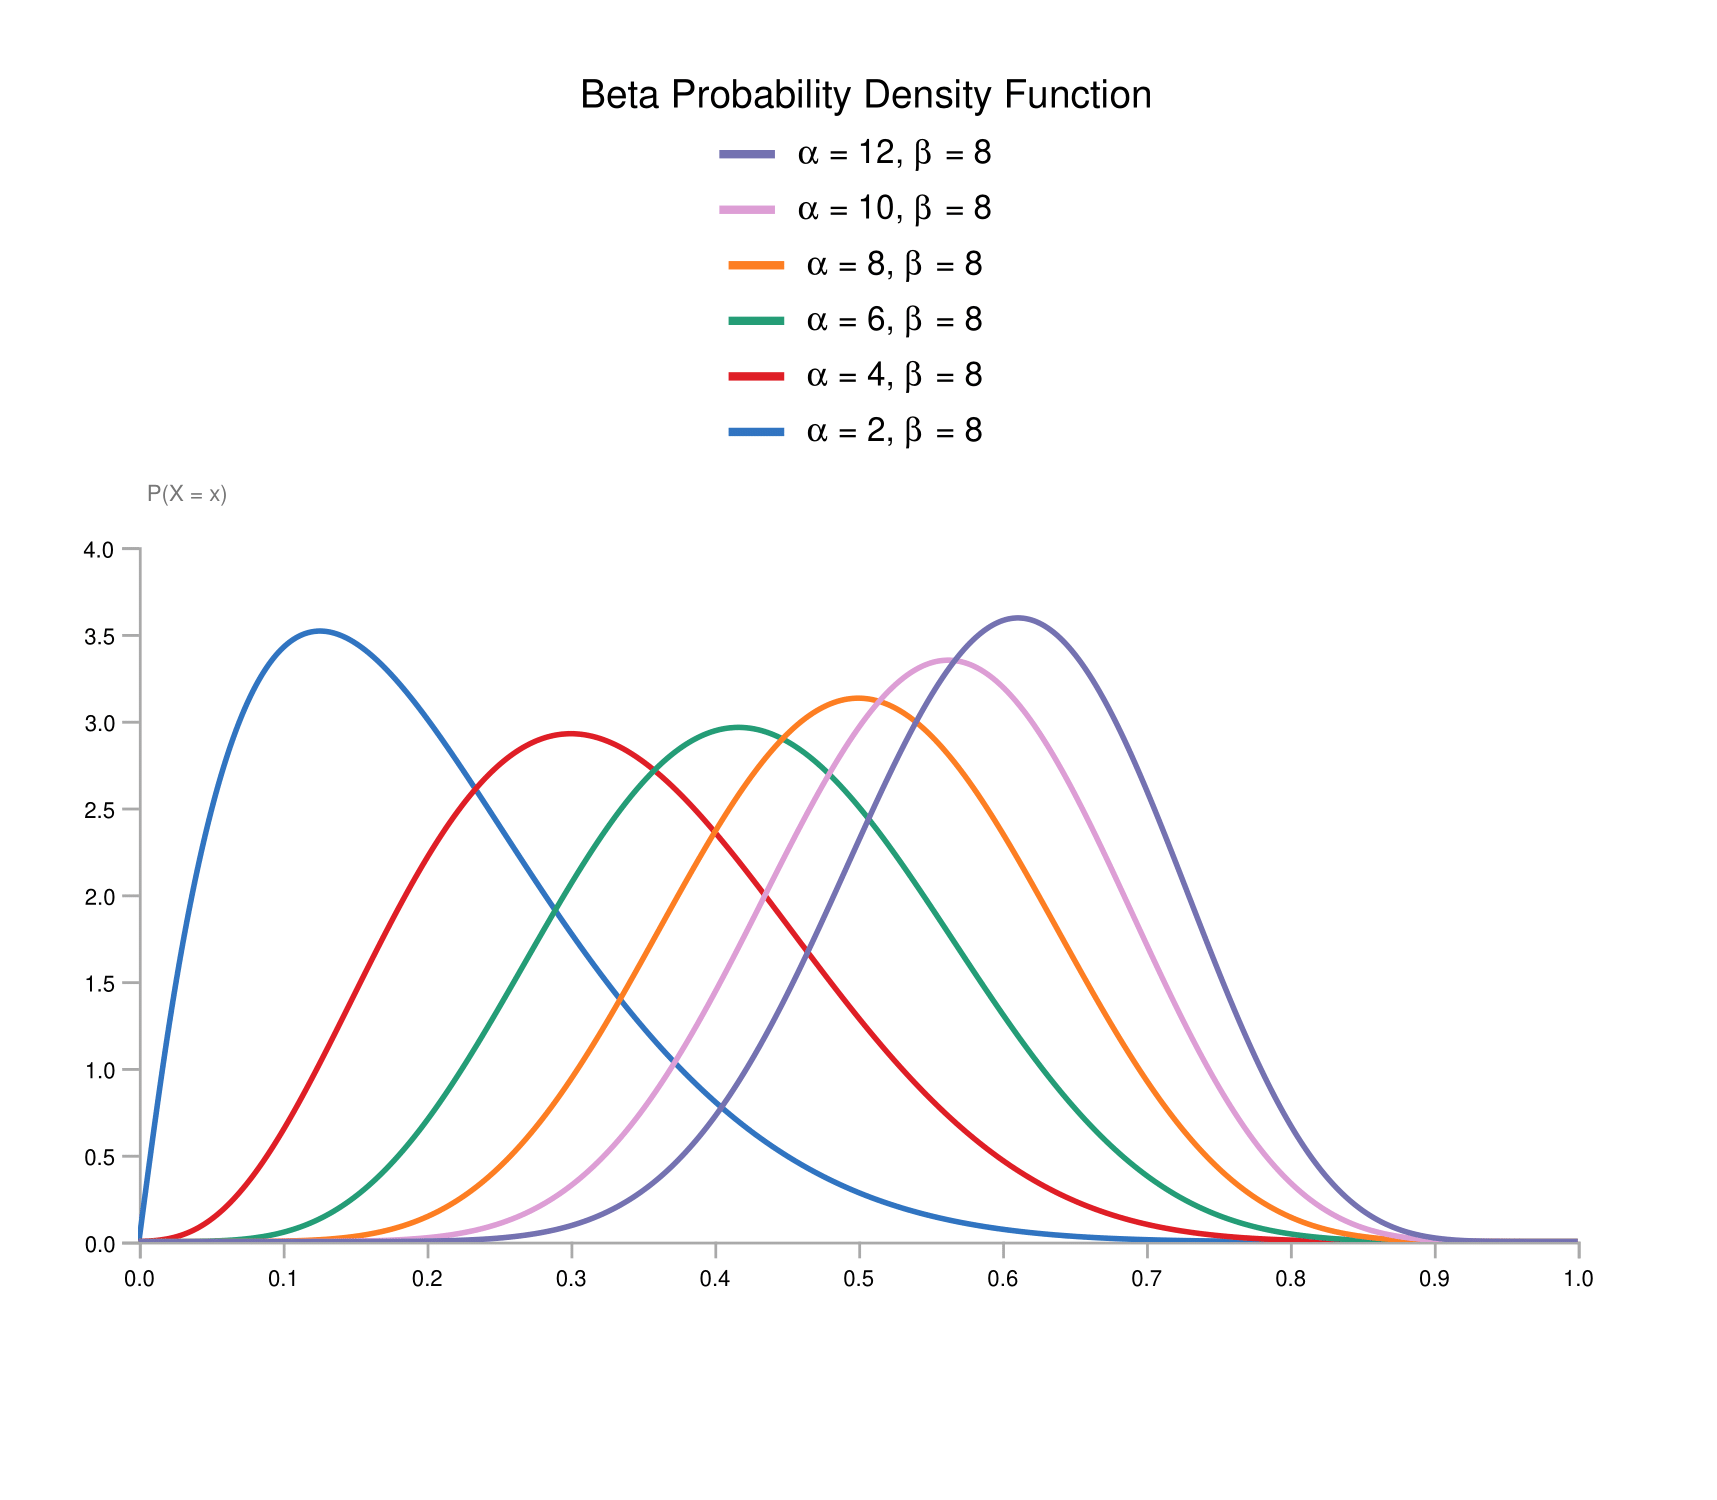
\includegraphics[width=6cm]{./images/chart (1)-1.png}\quad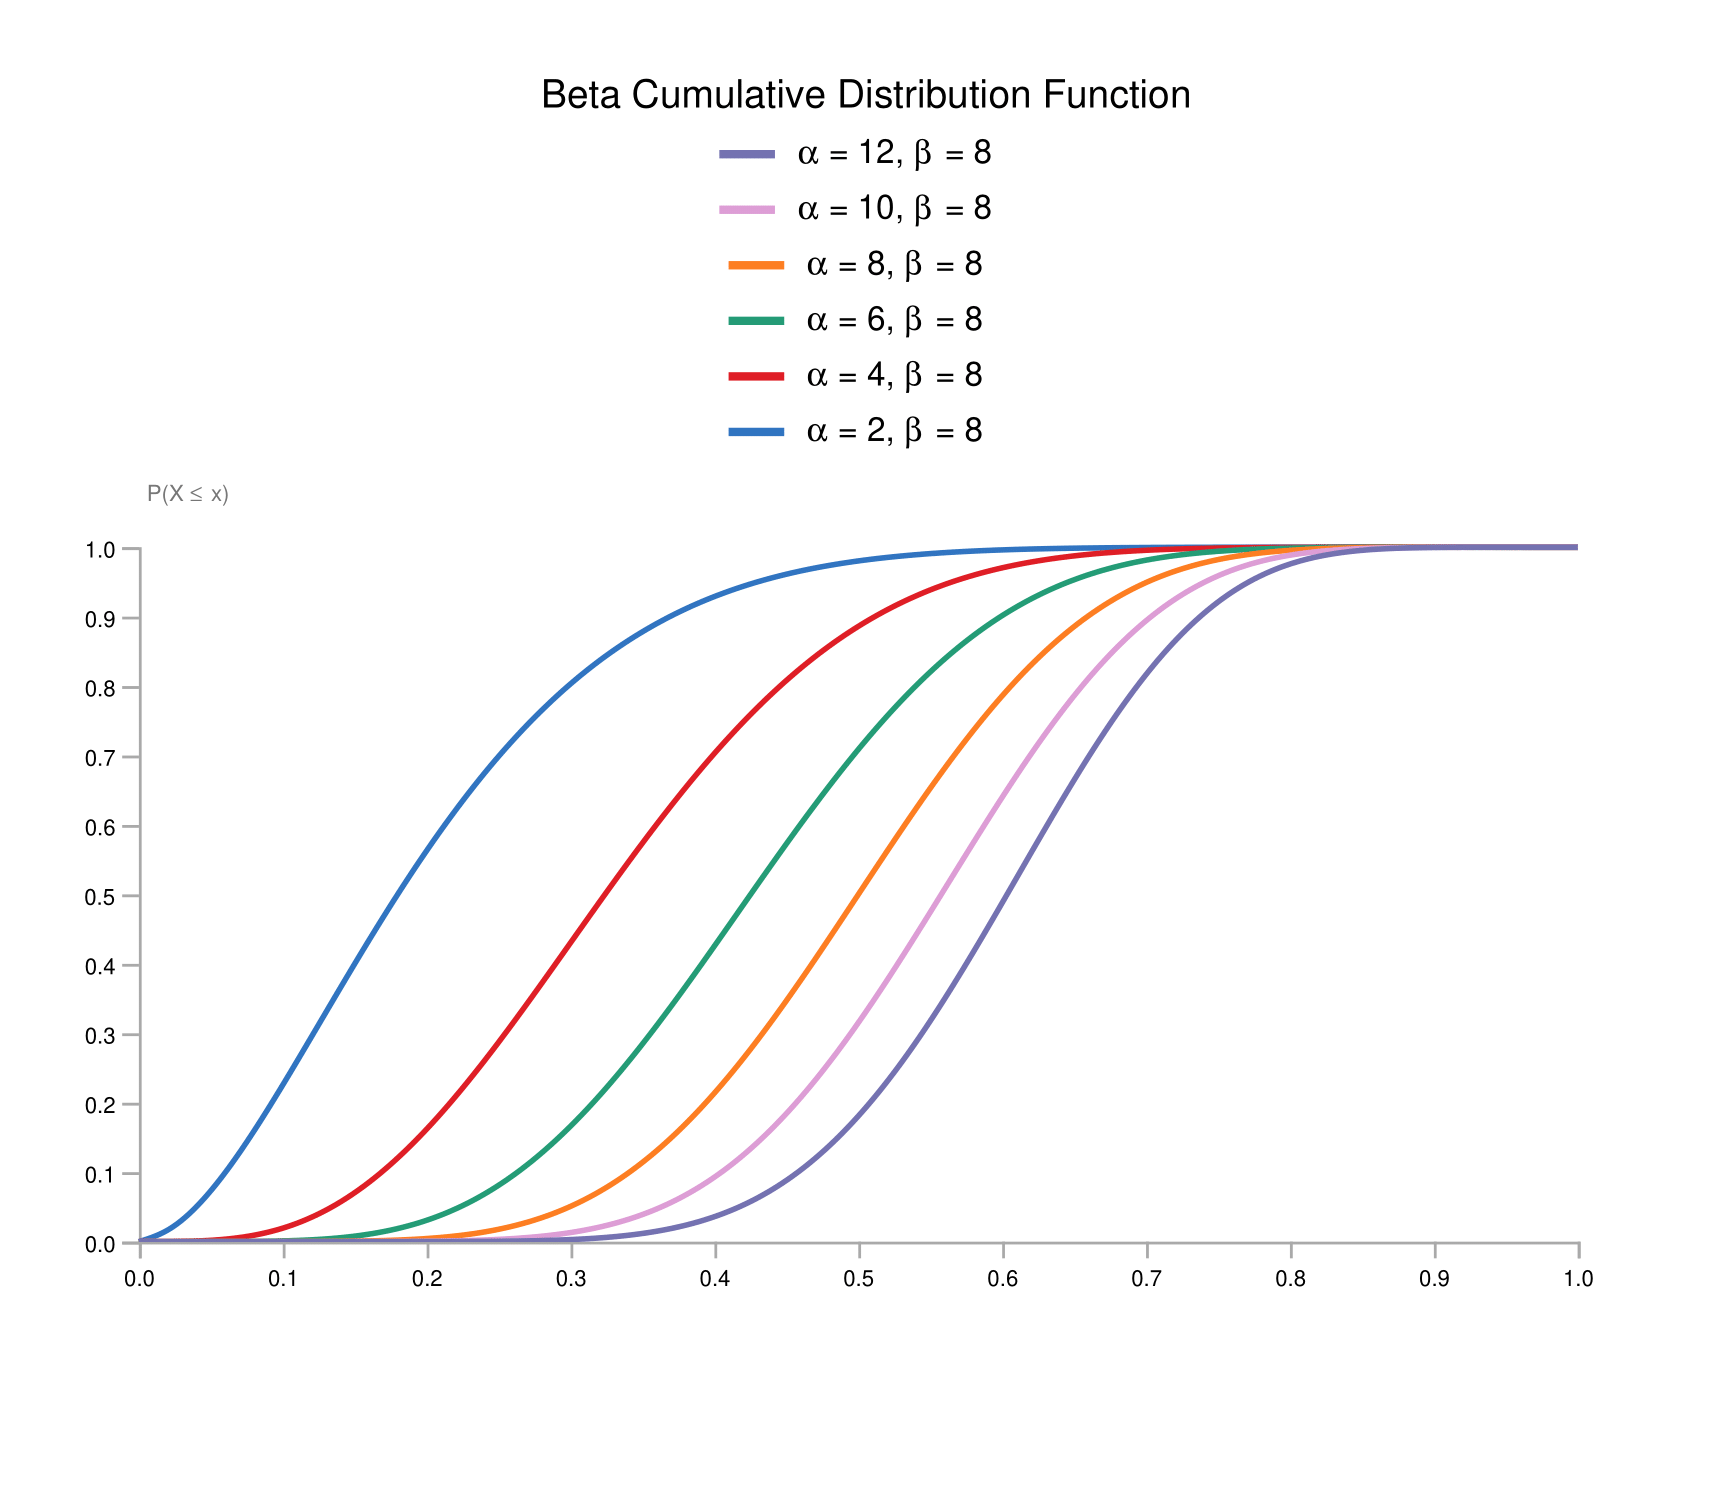
\includegraphics[width=6cm]{./images/chart (2)-1.png}
	\caption{Beta distribution description, PDF and CDF}
	\label{beta}
\end{figure}

\subsection{Synthetic C}

$Tmax = 5, 10, 20, 40, 70, 110, 160, 210$
N\_runs = 20 for each configuration

\begin{table}[H]
	\centering
	\caption{arm descriptions synthetic C}
	\begin{tabular}{|l||l|l|l|l|l|l|l|l|l|l|l|} 
		\hline
		\textbf{arm} & \textbf{R} & $\boldsymbol{\alpha}$ & $\boldsymbol{\beta}$ & $\boldsymbol{\mu_5}$ & $\boldsymbol{\mu_{10}}$ & $\boldsymbol{\mu_{20}}$ & $\boldsymbol{\mu_{40}}$ & $\boldsymbol{\mu_{70}}$ & $\boldsymbol{\mu_{110}}$& $\boldsymbol{\mu_{160}}$& $\boldsymbol{\mu_{210}}$ \\ 
		\hline
		$a_0$     & 6          & 2        & 8       &    & & & & & & &                \\ 
		\hline
		$a_1$     & 5          & 4        & 8       &    & & & & & & &                   \\ 
		\hline
		$a_2$     & 4          & 6        & 8       &          & & & & & & &           \\ 
		\hline
		$a_3$     & 3          & 8        & 8       &                 & & & & & & &     \\ 
		\hline
		$a_4$     & 2          & 10        & 8       & & & & & & & &                  \\ 
		\hline
		${a_5}$     & 1          & 12        & 8       &      & & & & &  &&                \\                 
		\hline
	\end{tabular}
\end{table}

\section{Results}

\begin{figure}[h]
	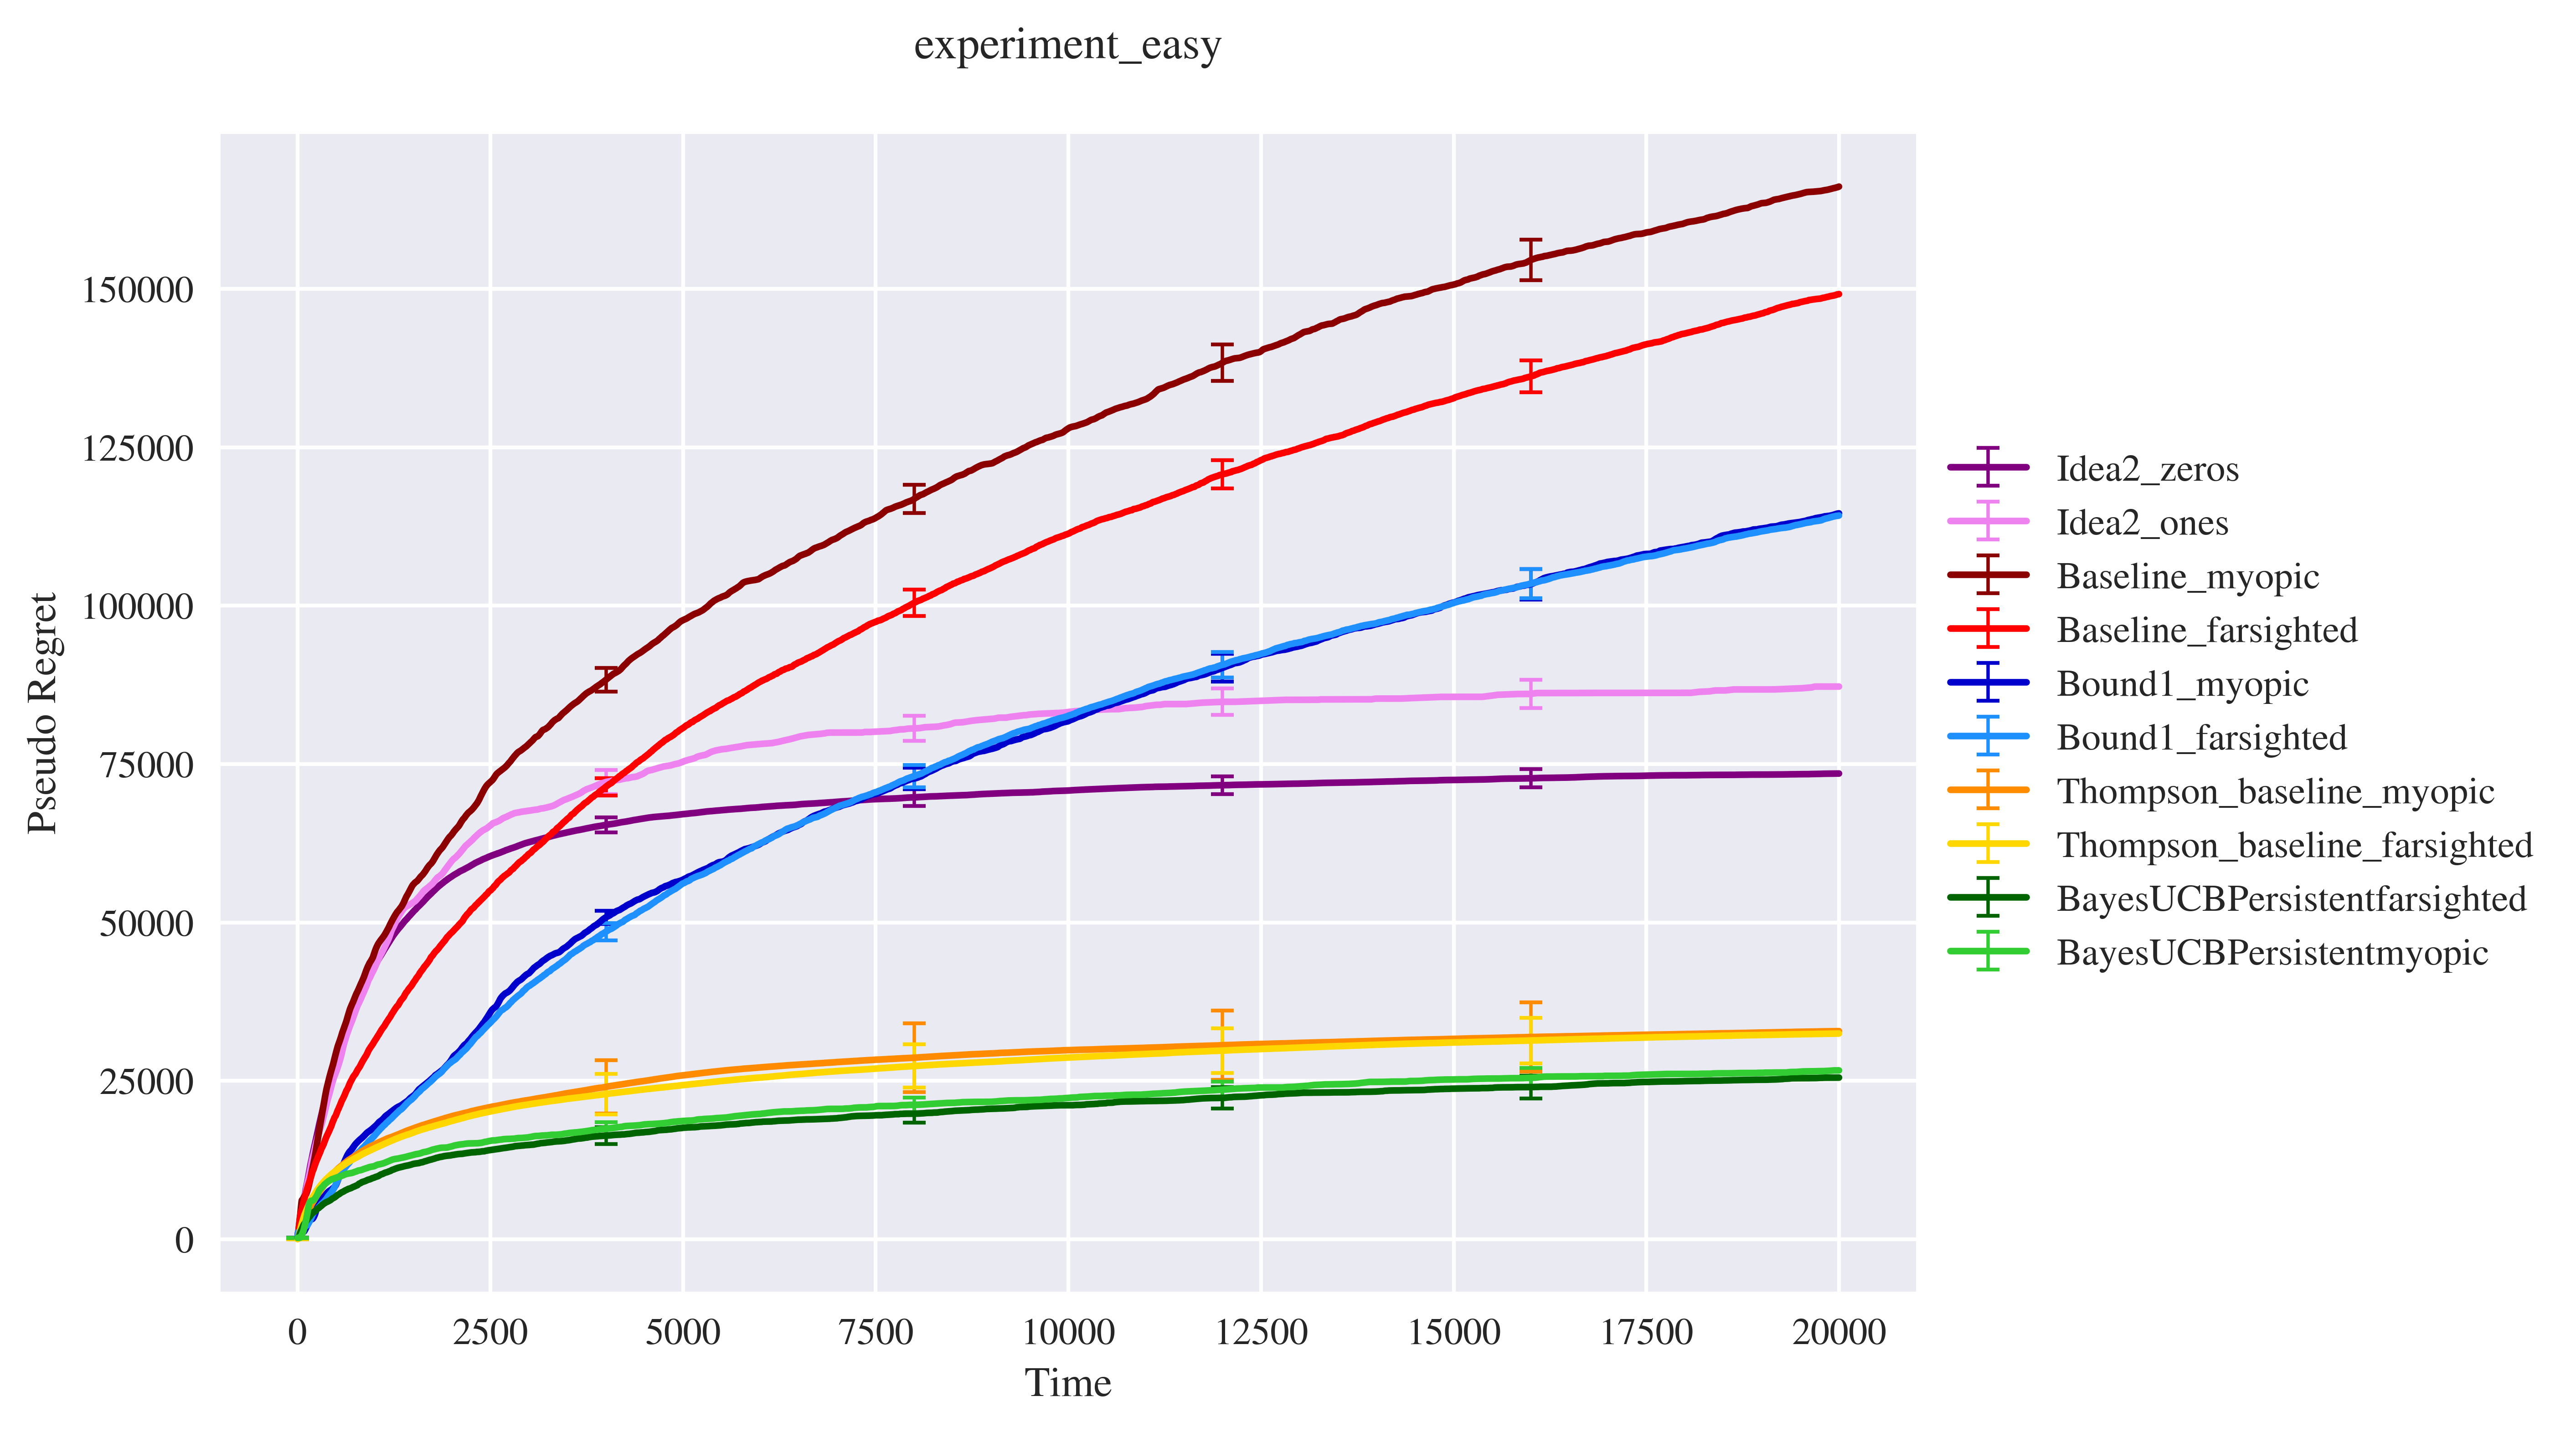
\includegraphics[width=16cm]{./images/experiment_easy ANALYTICS.png}
	\centering	
	\caption{SYNTHETIC A pseudo regret: beta uniformi (R: 1...10) 50 runs Tmax=50}
\end{figure}
\begin{figure}[h]
	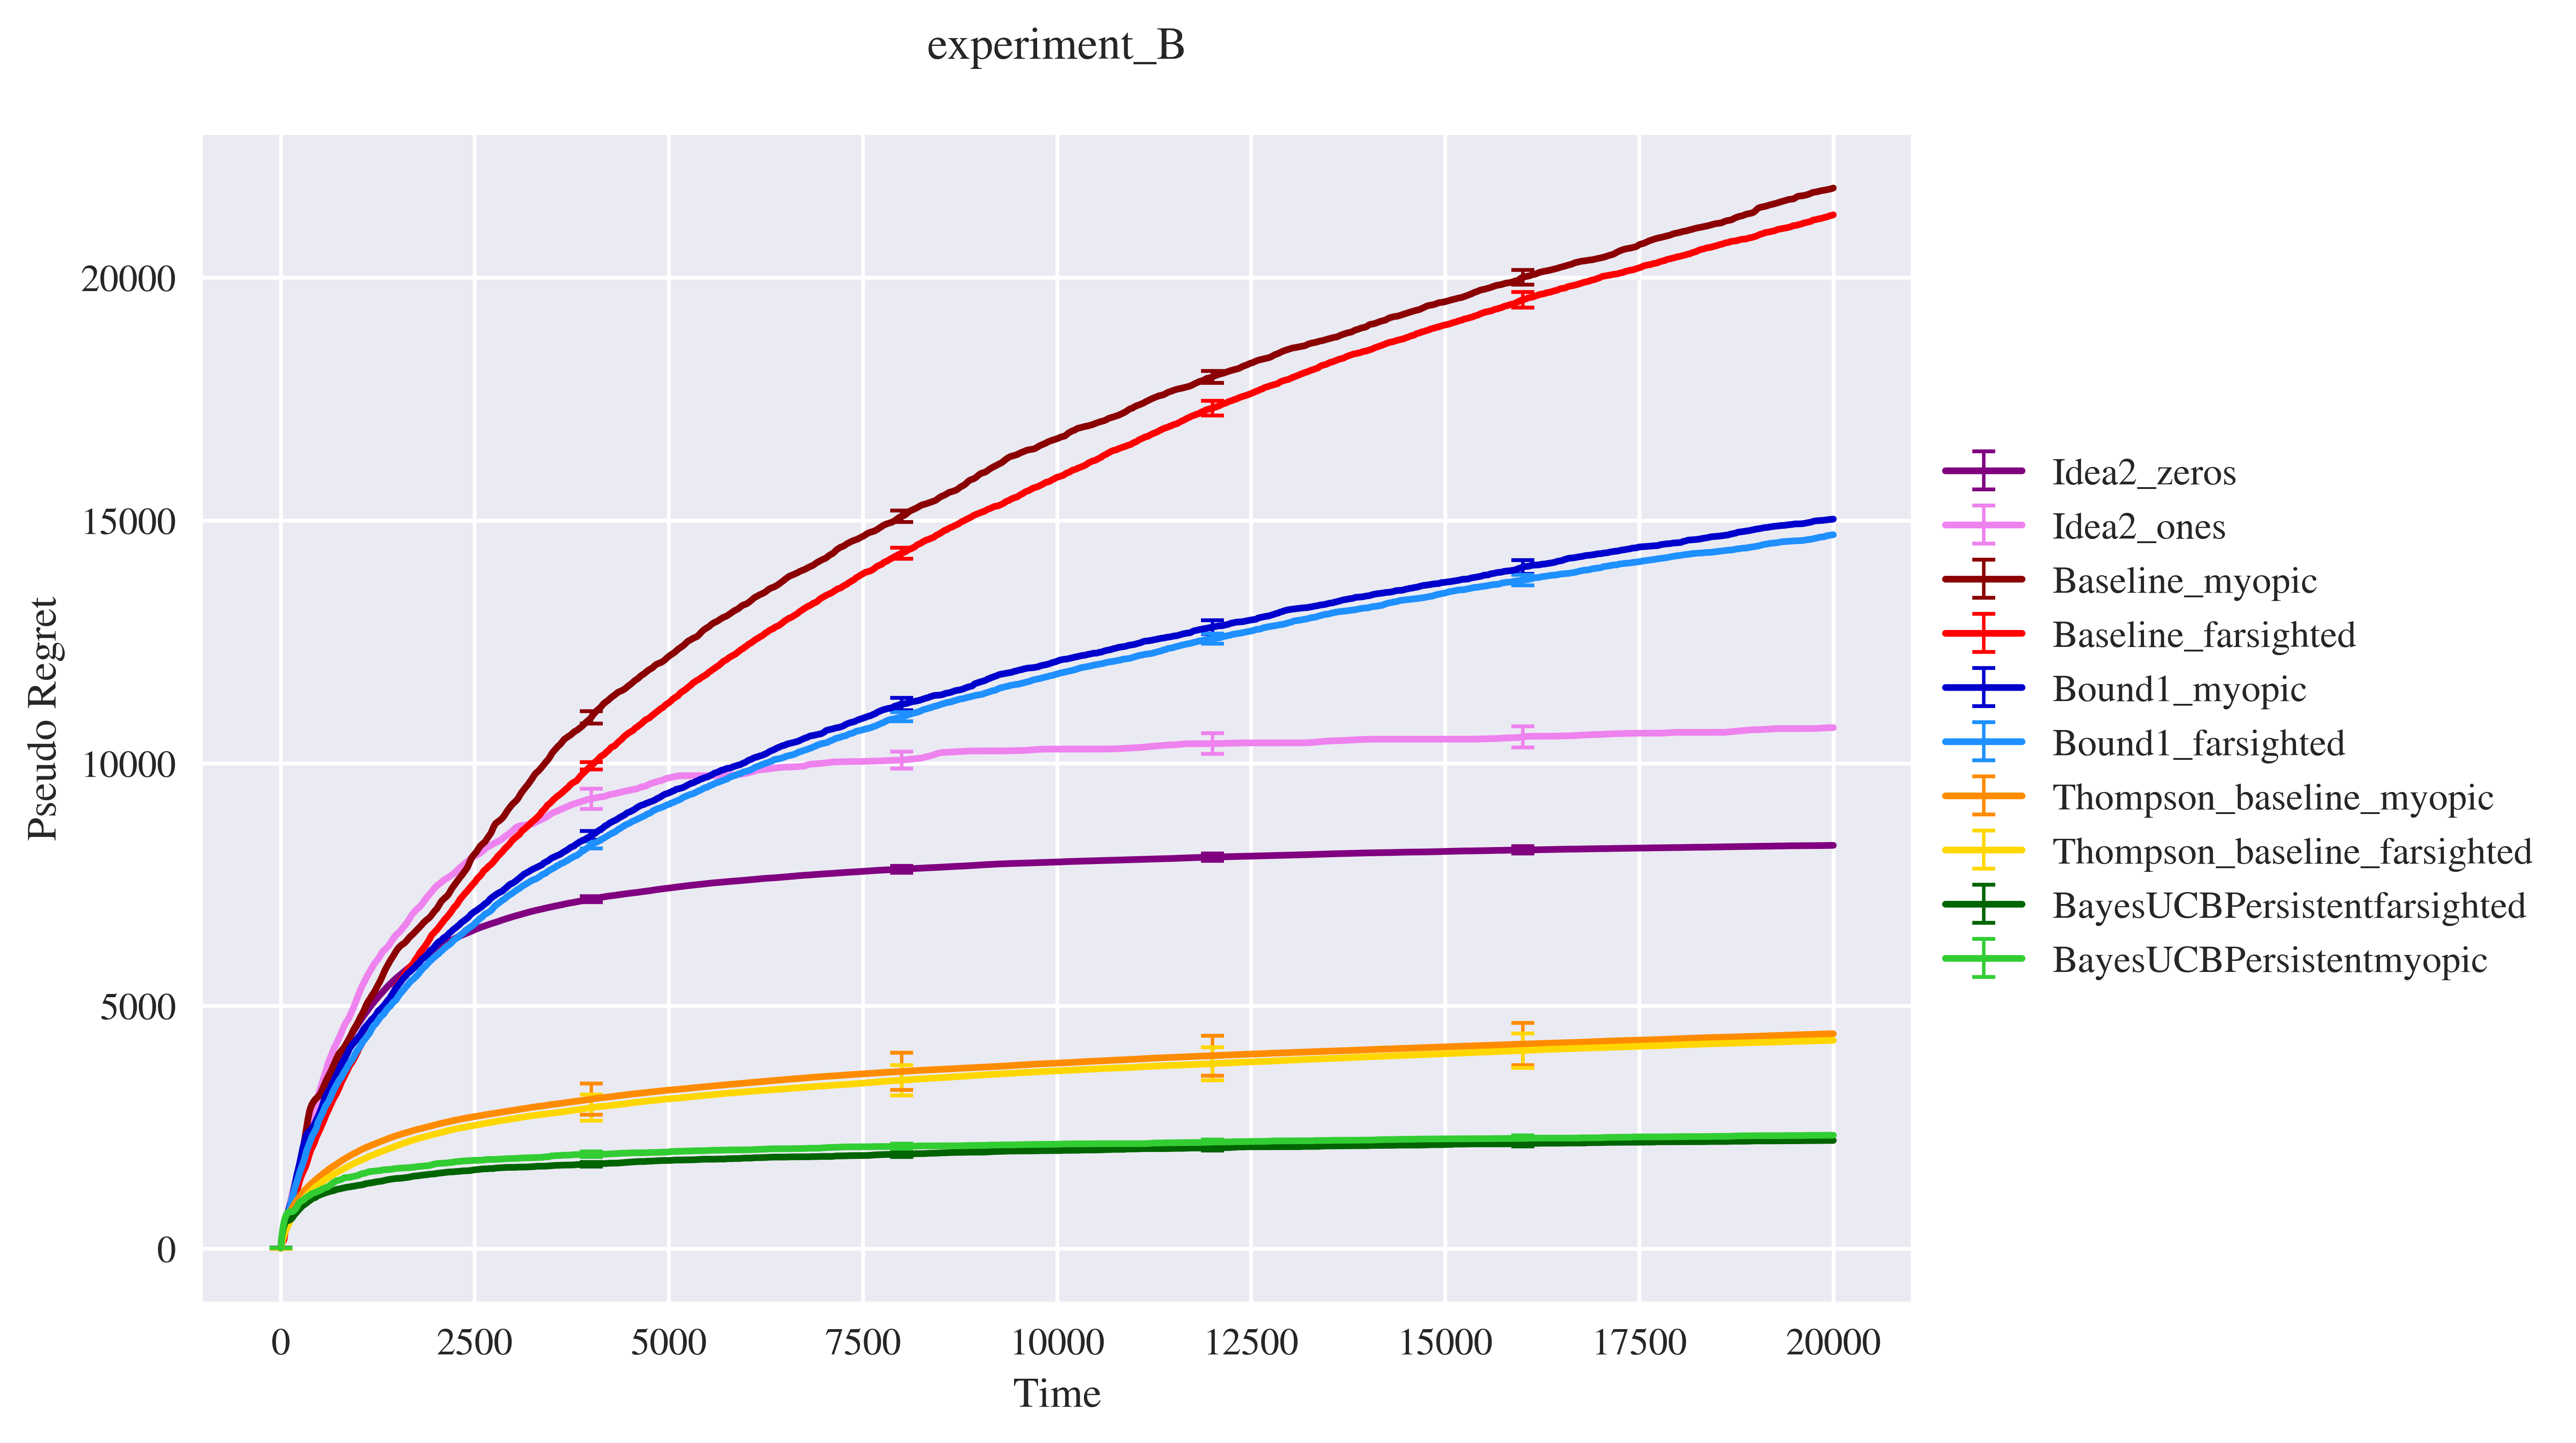
\includegraphics[width=16cm]{./images/experiment_B ANALYTICS.png}
	\centering	
	\caption{SYNTHETIC B pseudo regret: 50runs,  R fixed, Tmax=50, Beta "crescenti" }
\end{figure}

\begin{figure}
	\centering
	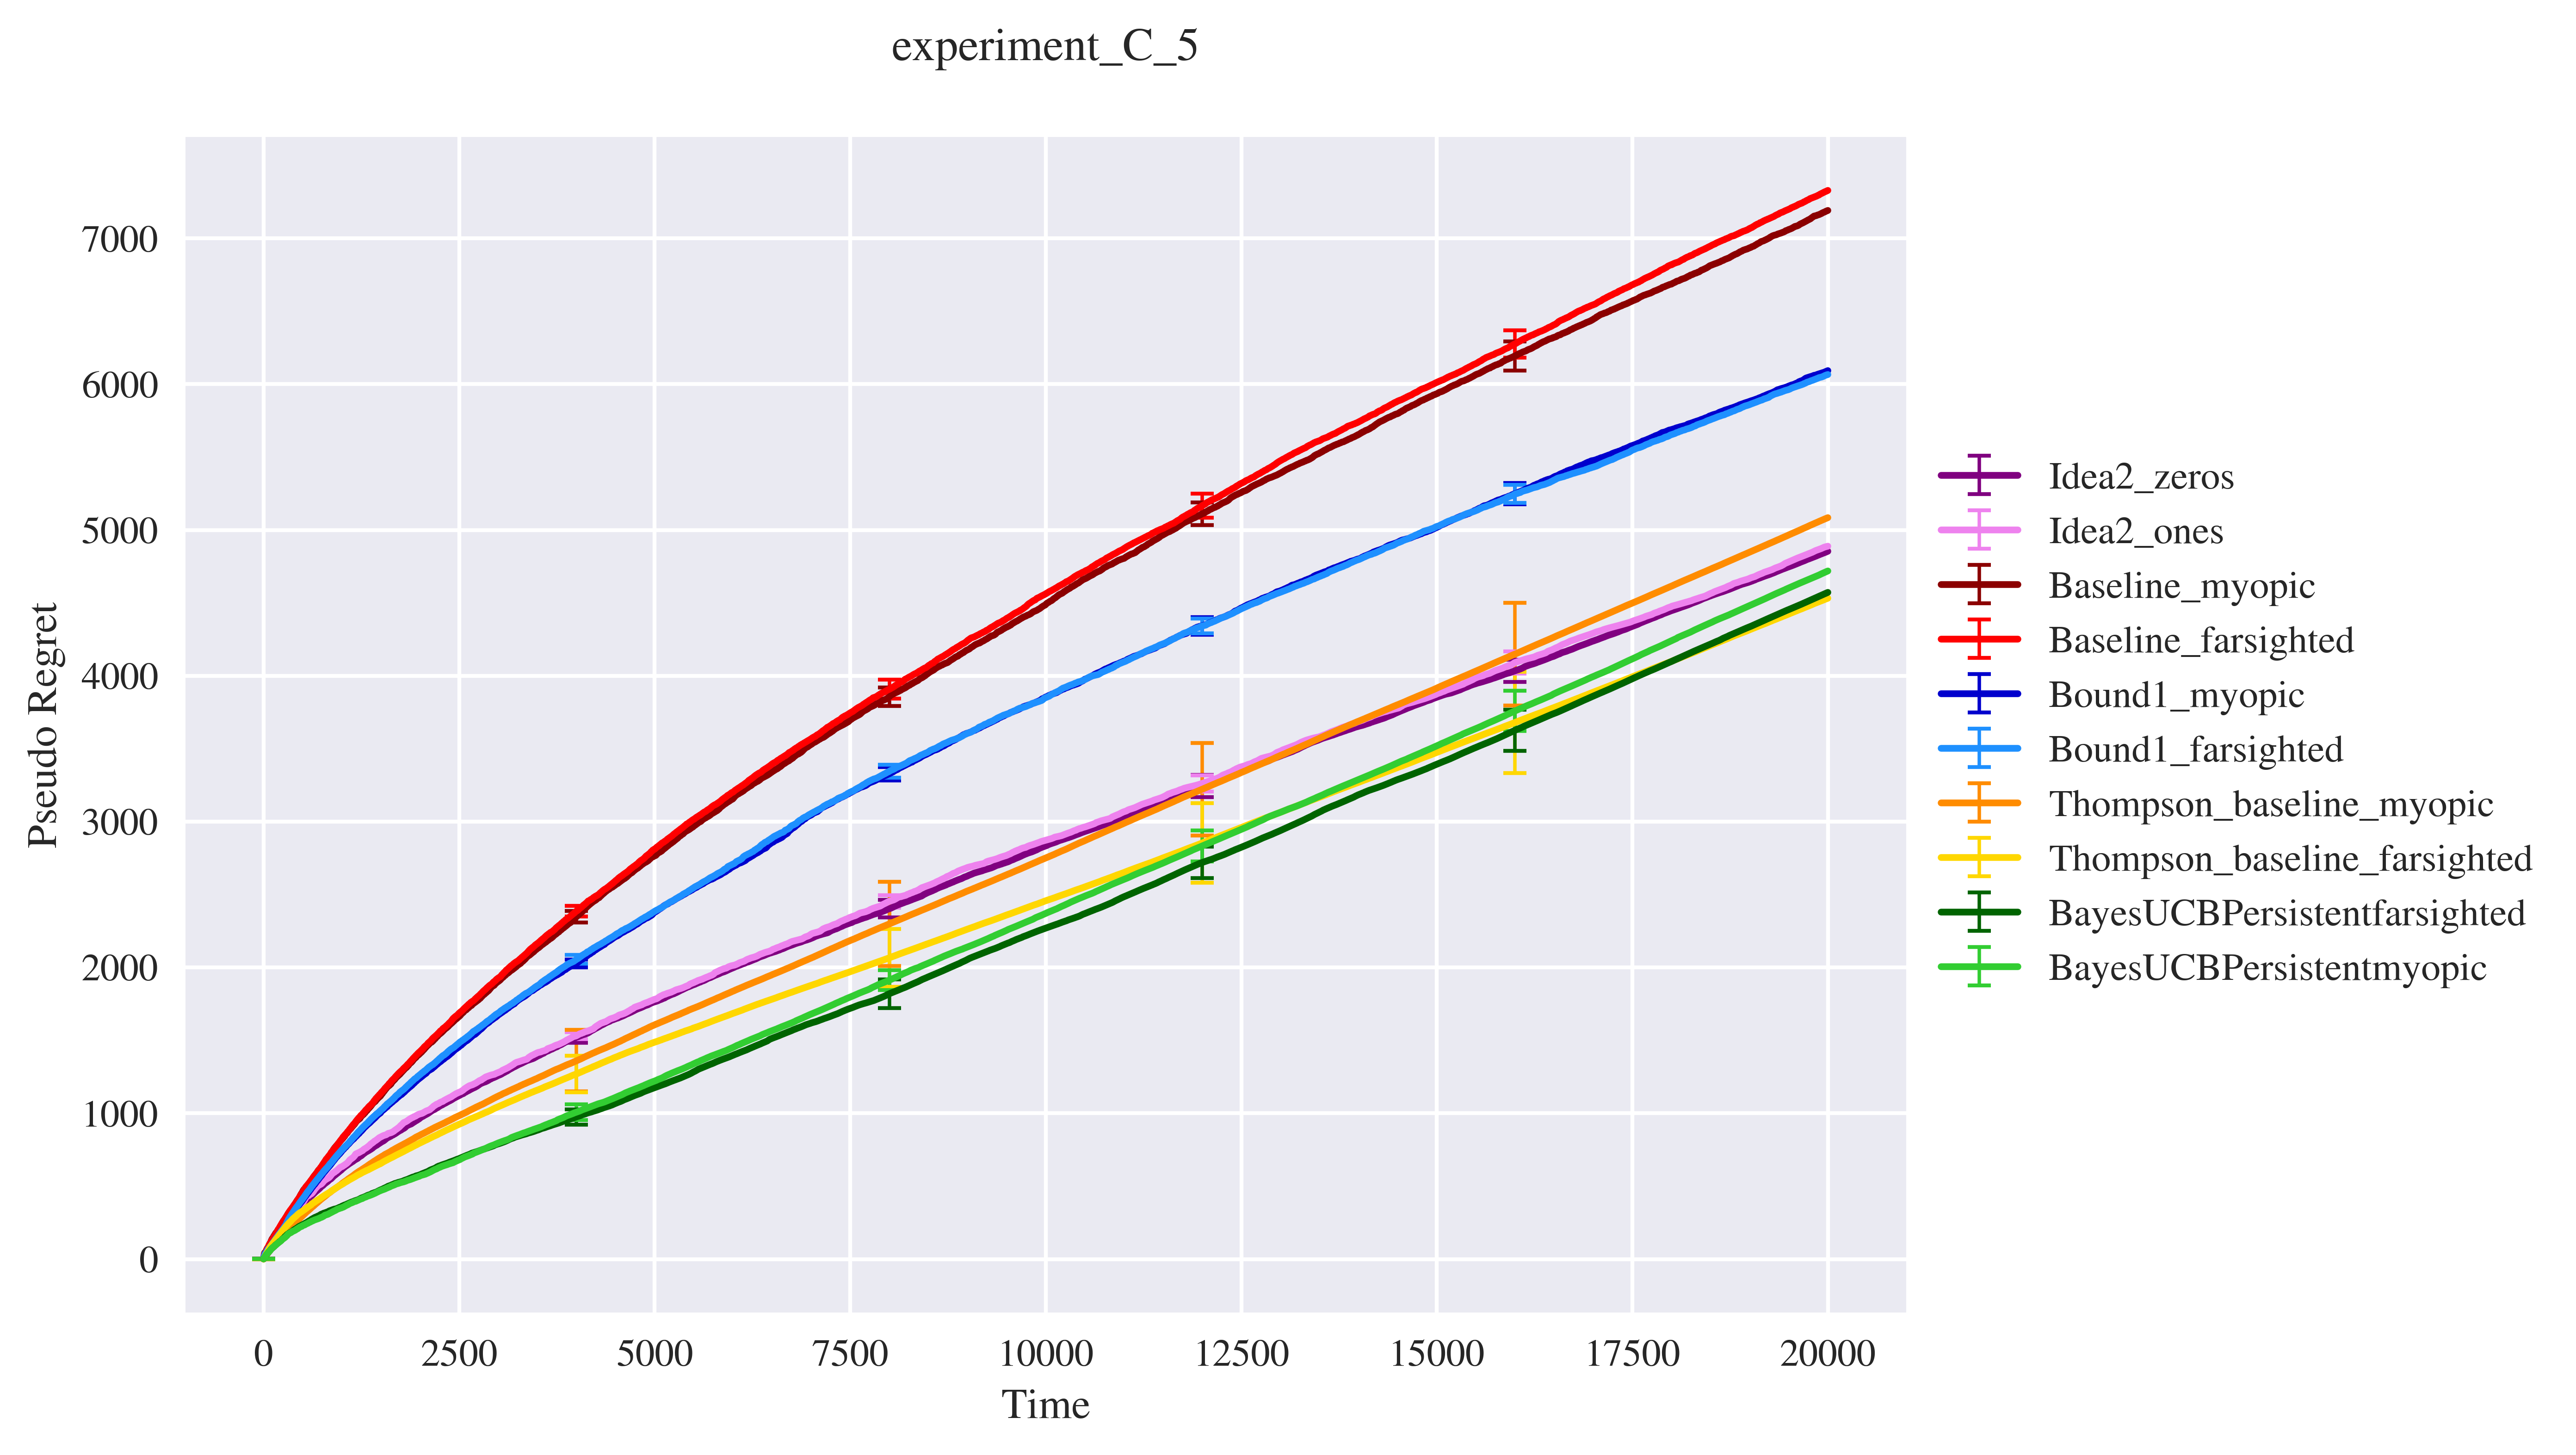
\includegraphics[width=6cm]{./images/C/experiment_C_5 ANALYTICS.png}\quad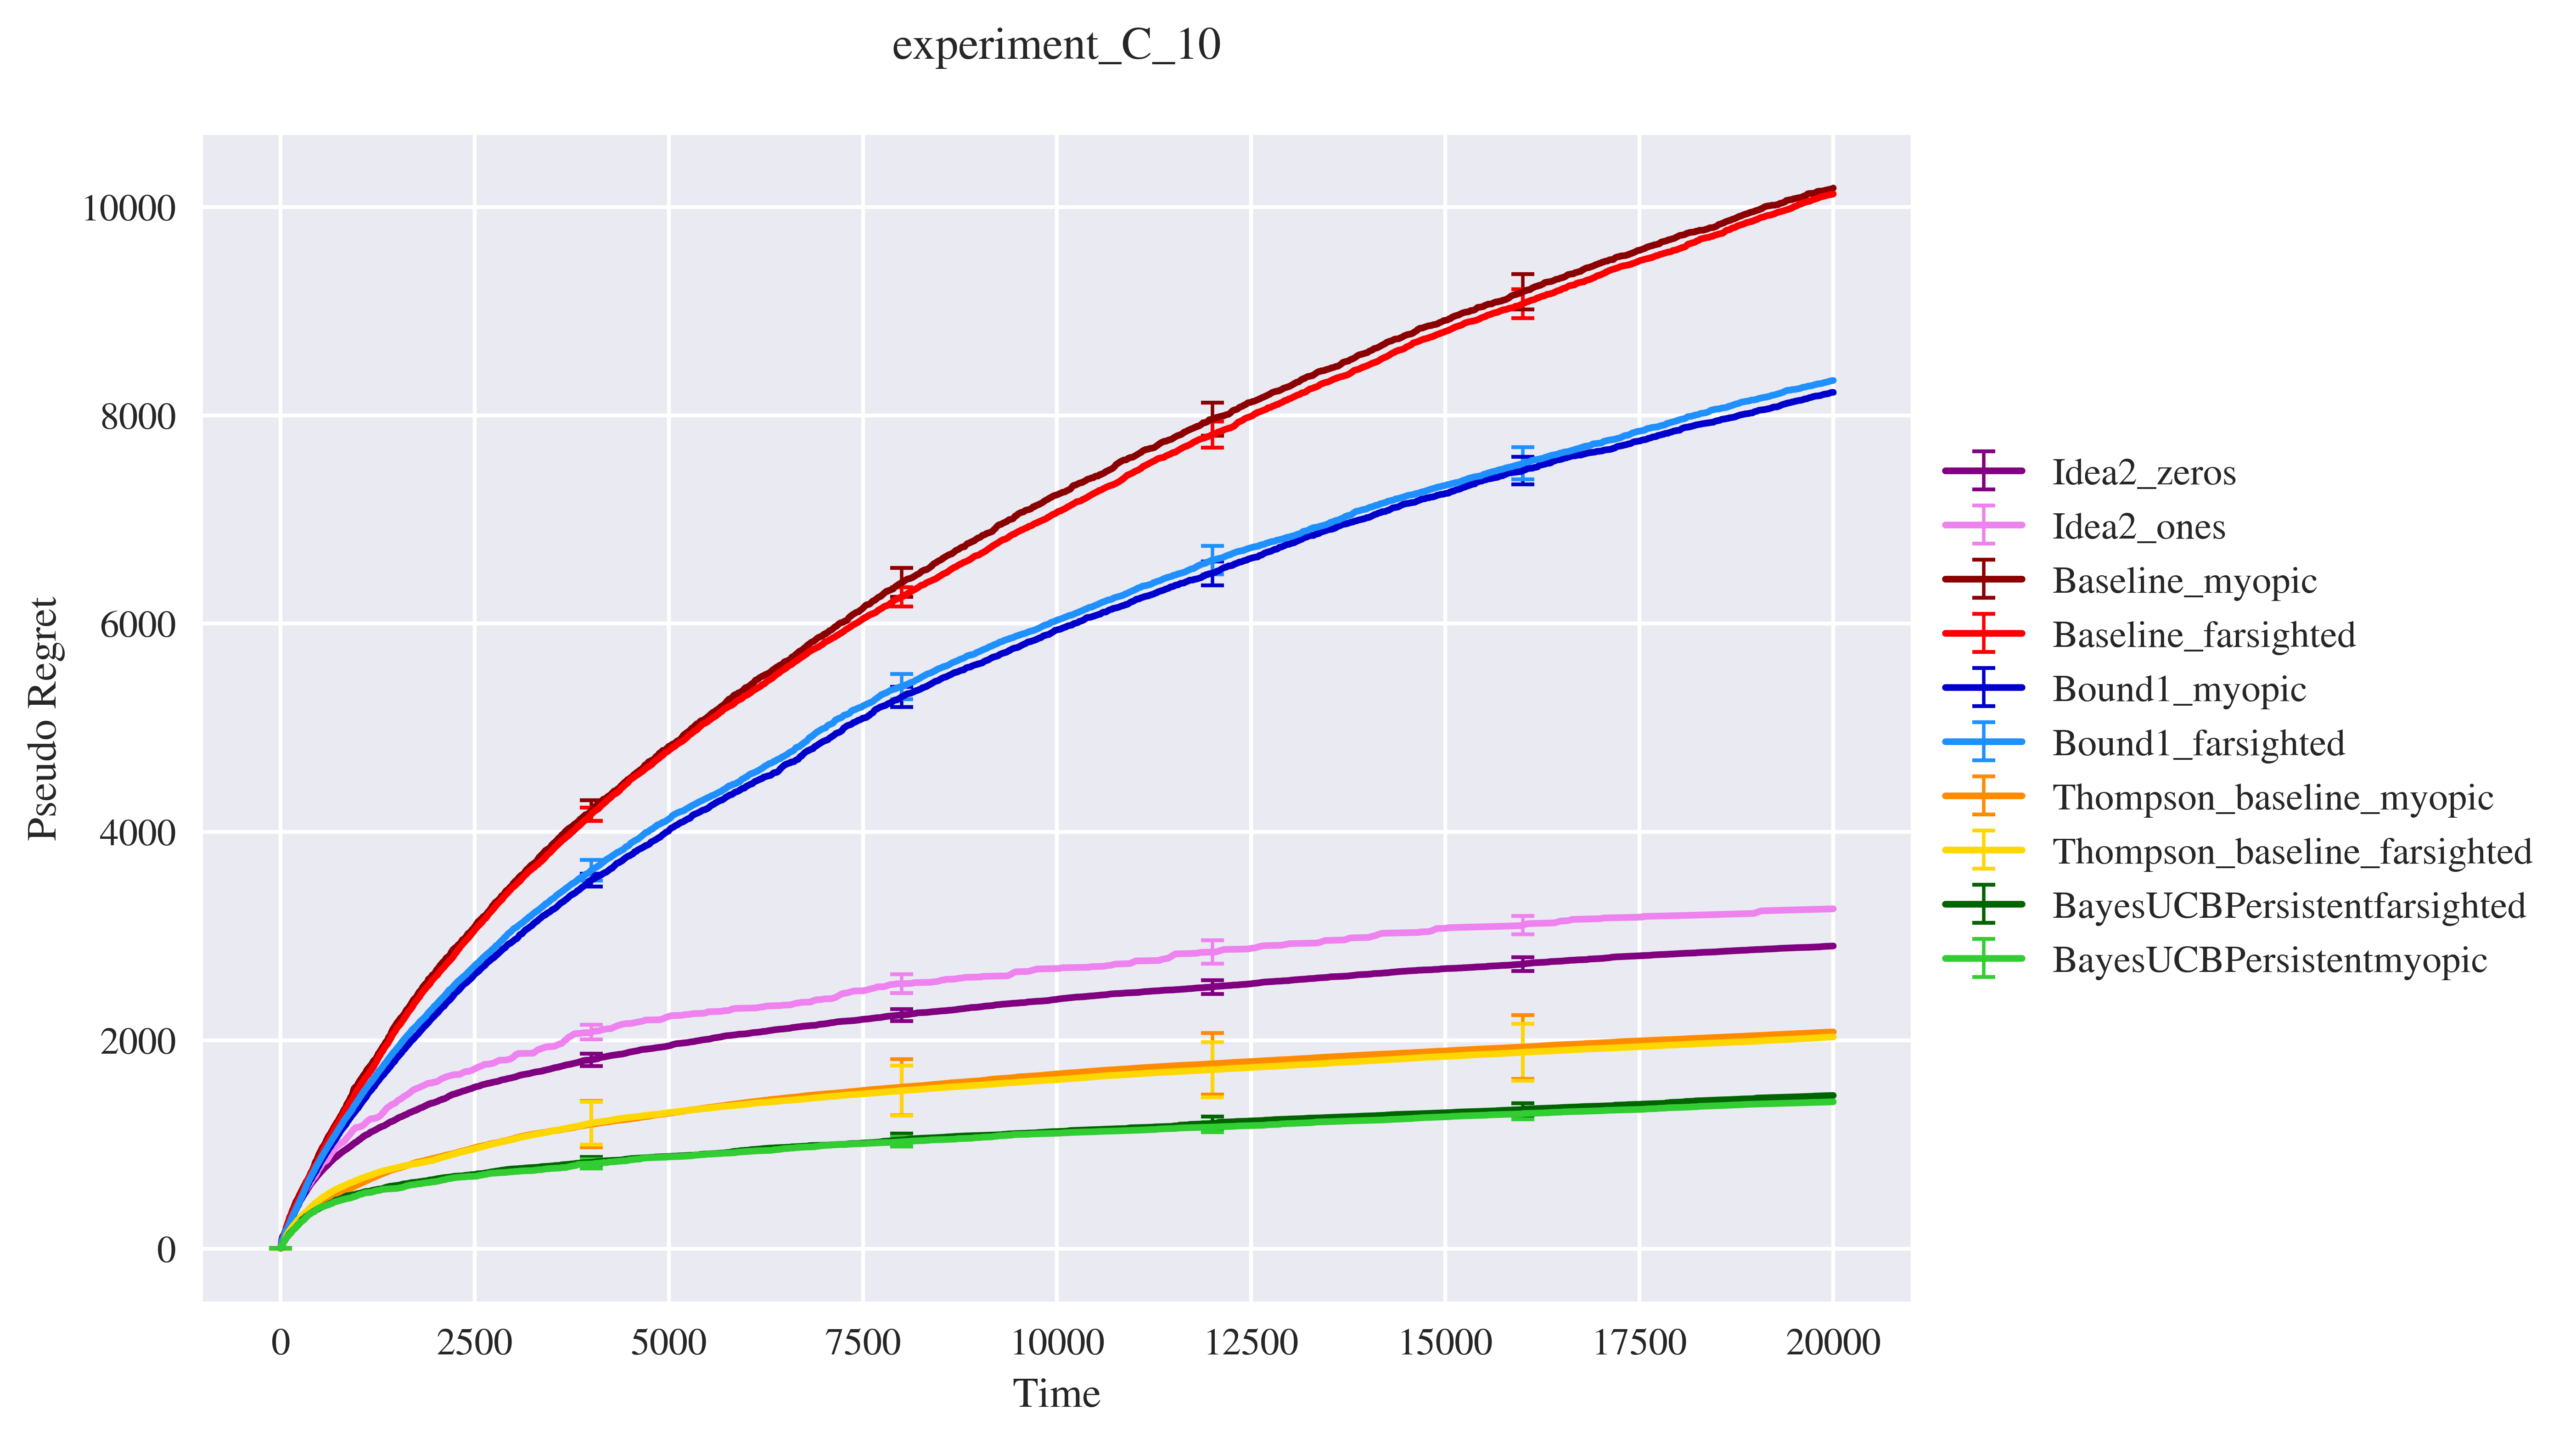
\includegraphics[width=6cm]{./images/C/experiment_C_10 ANALYTICS.png} 
	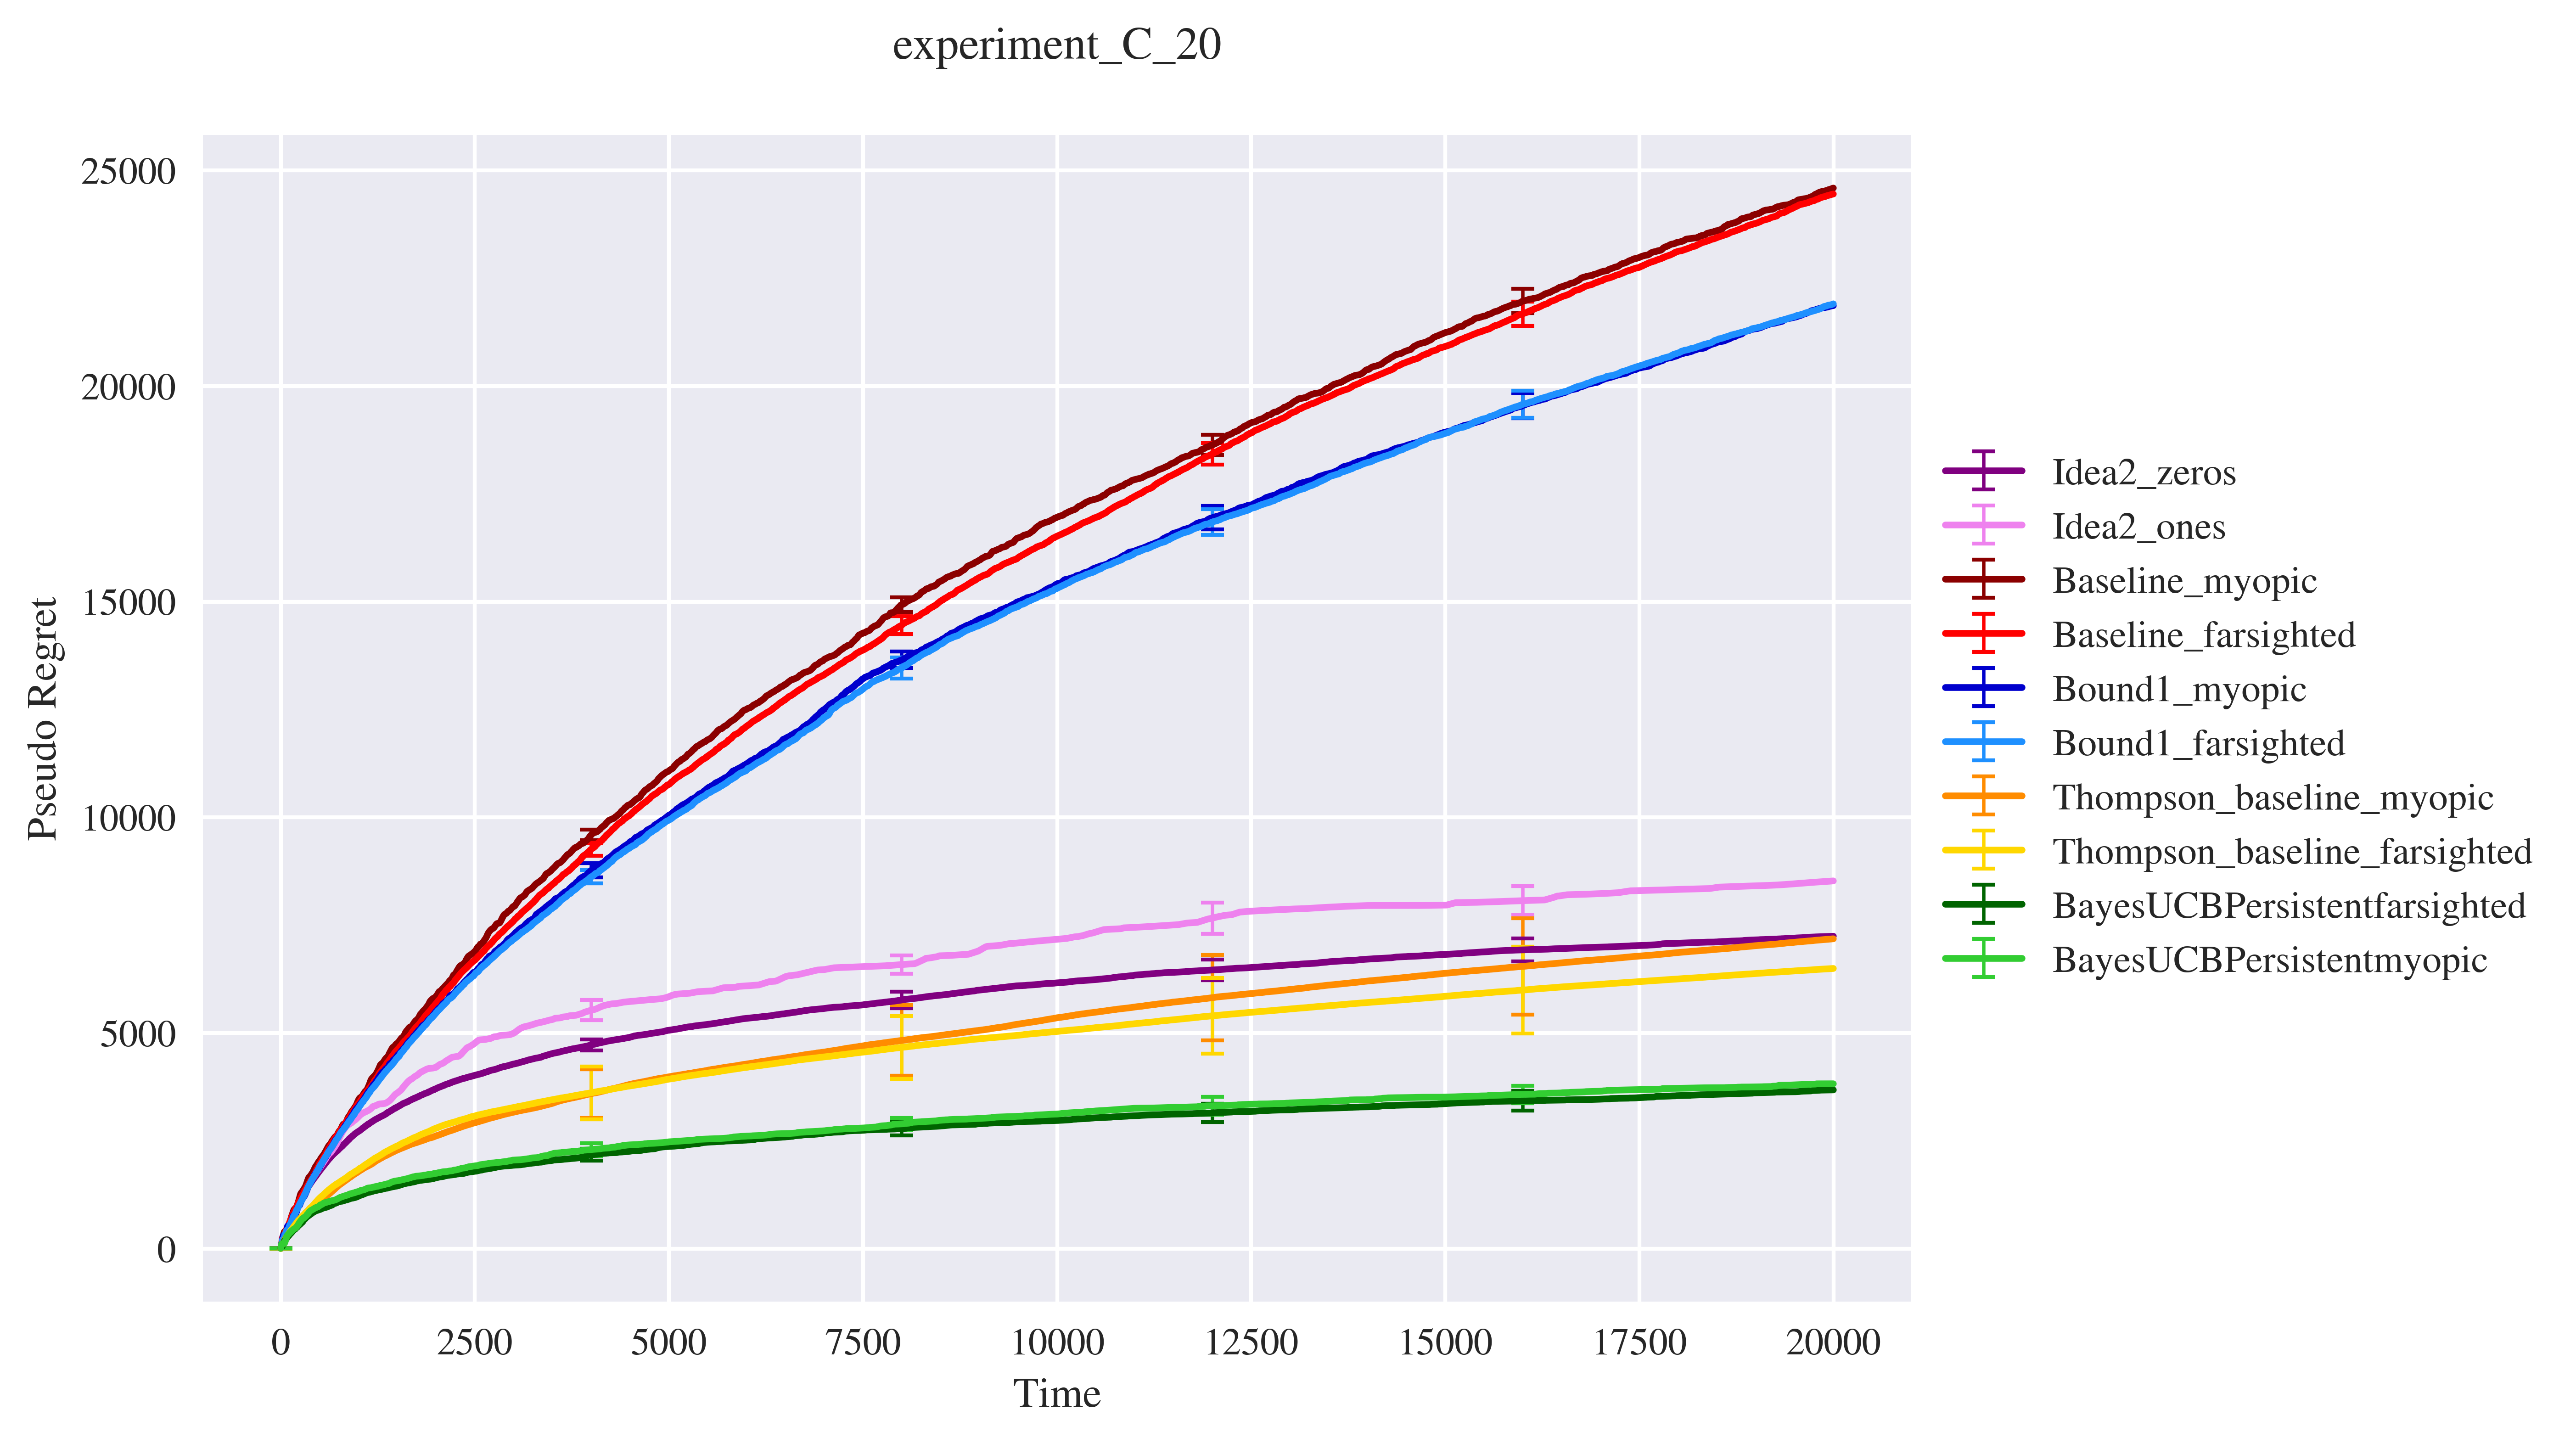
\includegraphics[width=6cm]{./images/C/experiment_C_20 ANALYTICS.png}\quad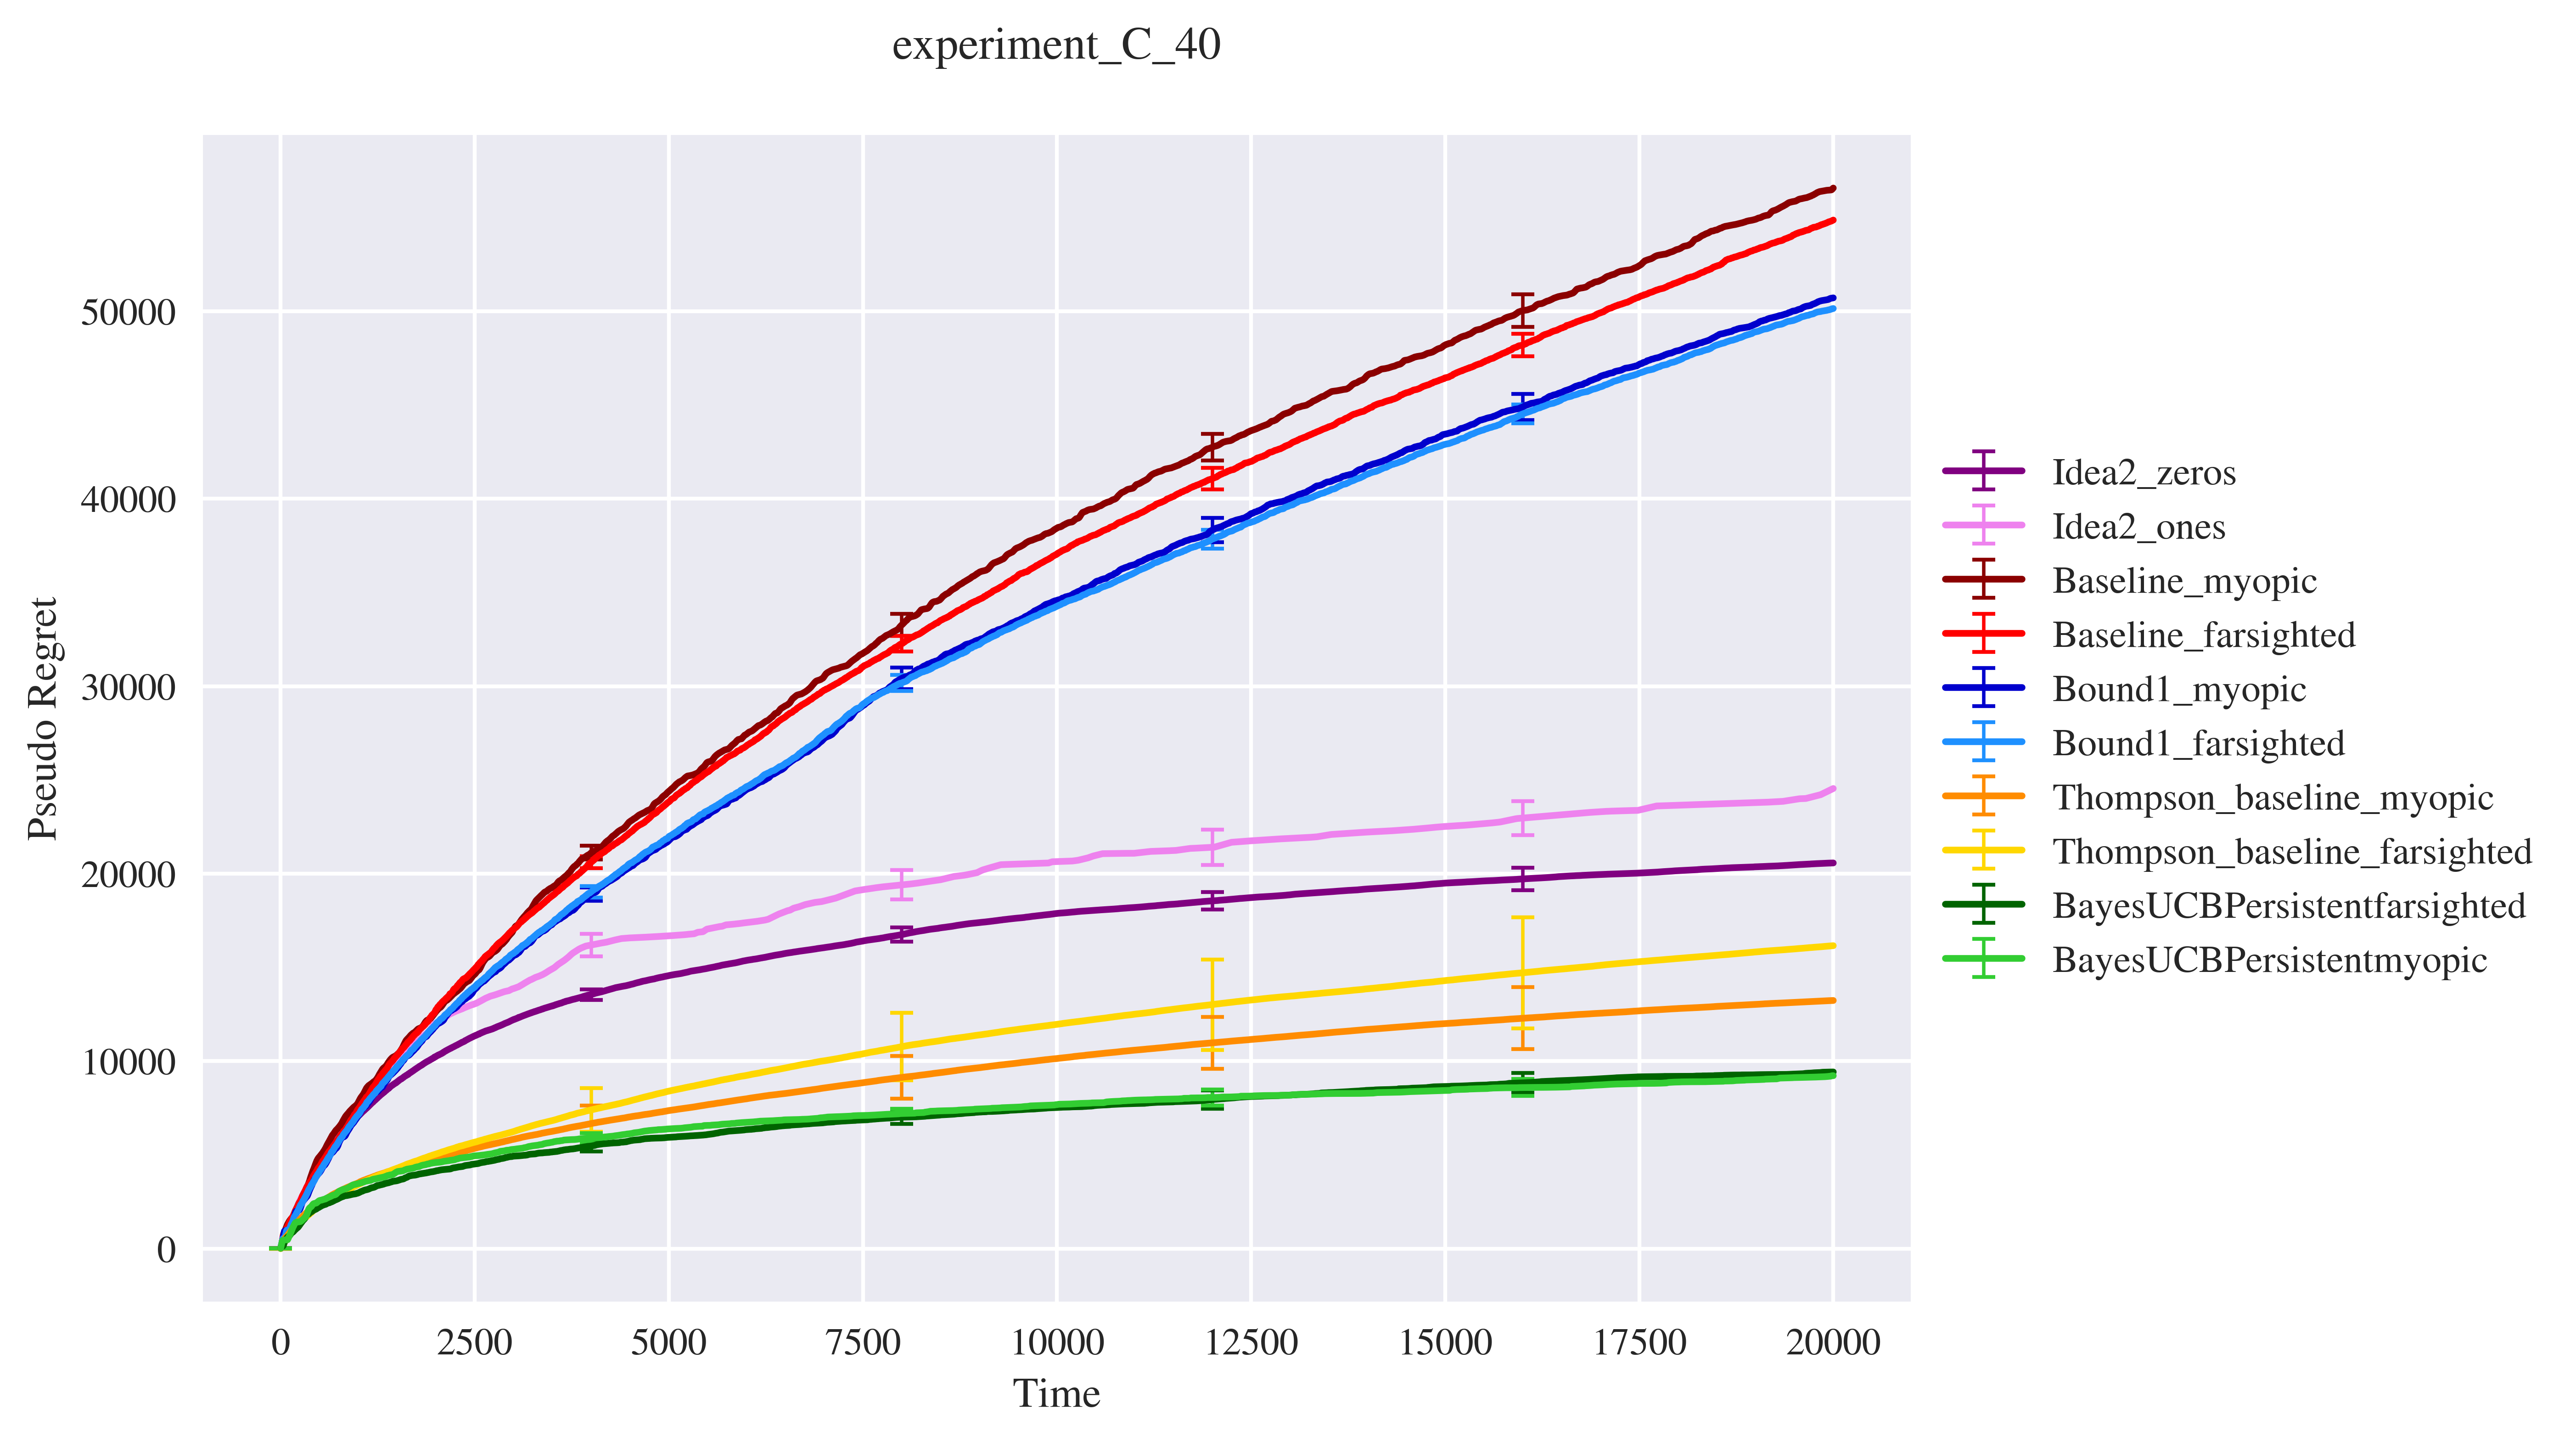
\includegraphics[width=6cm]{./images/C/experiment_C_40 ANALYTICS.png}
	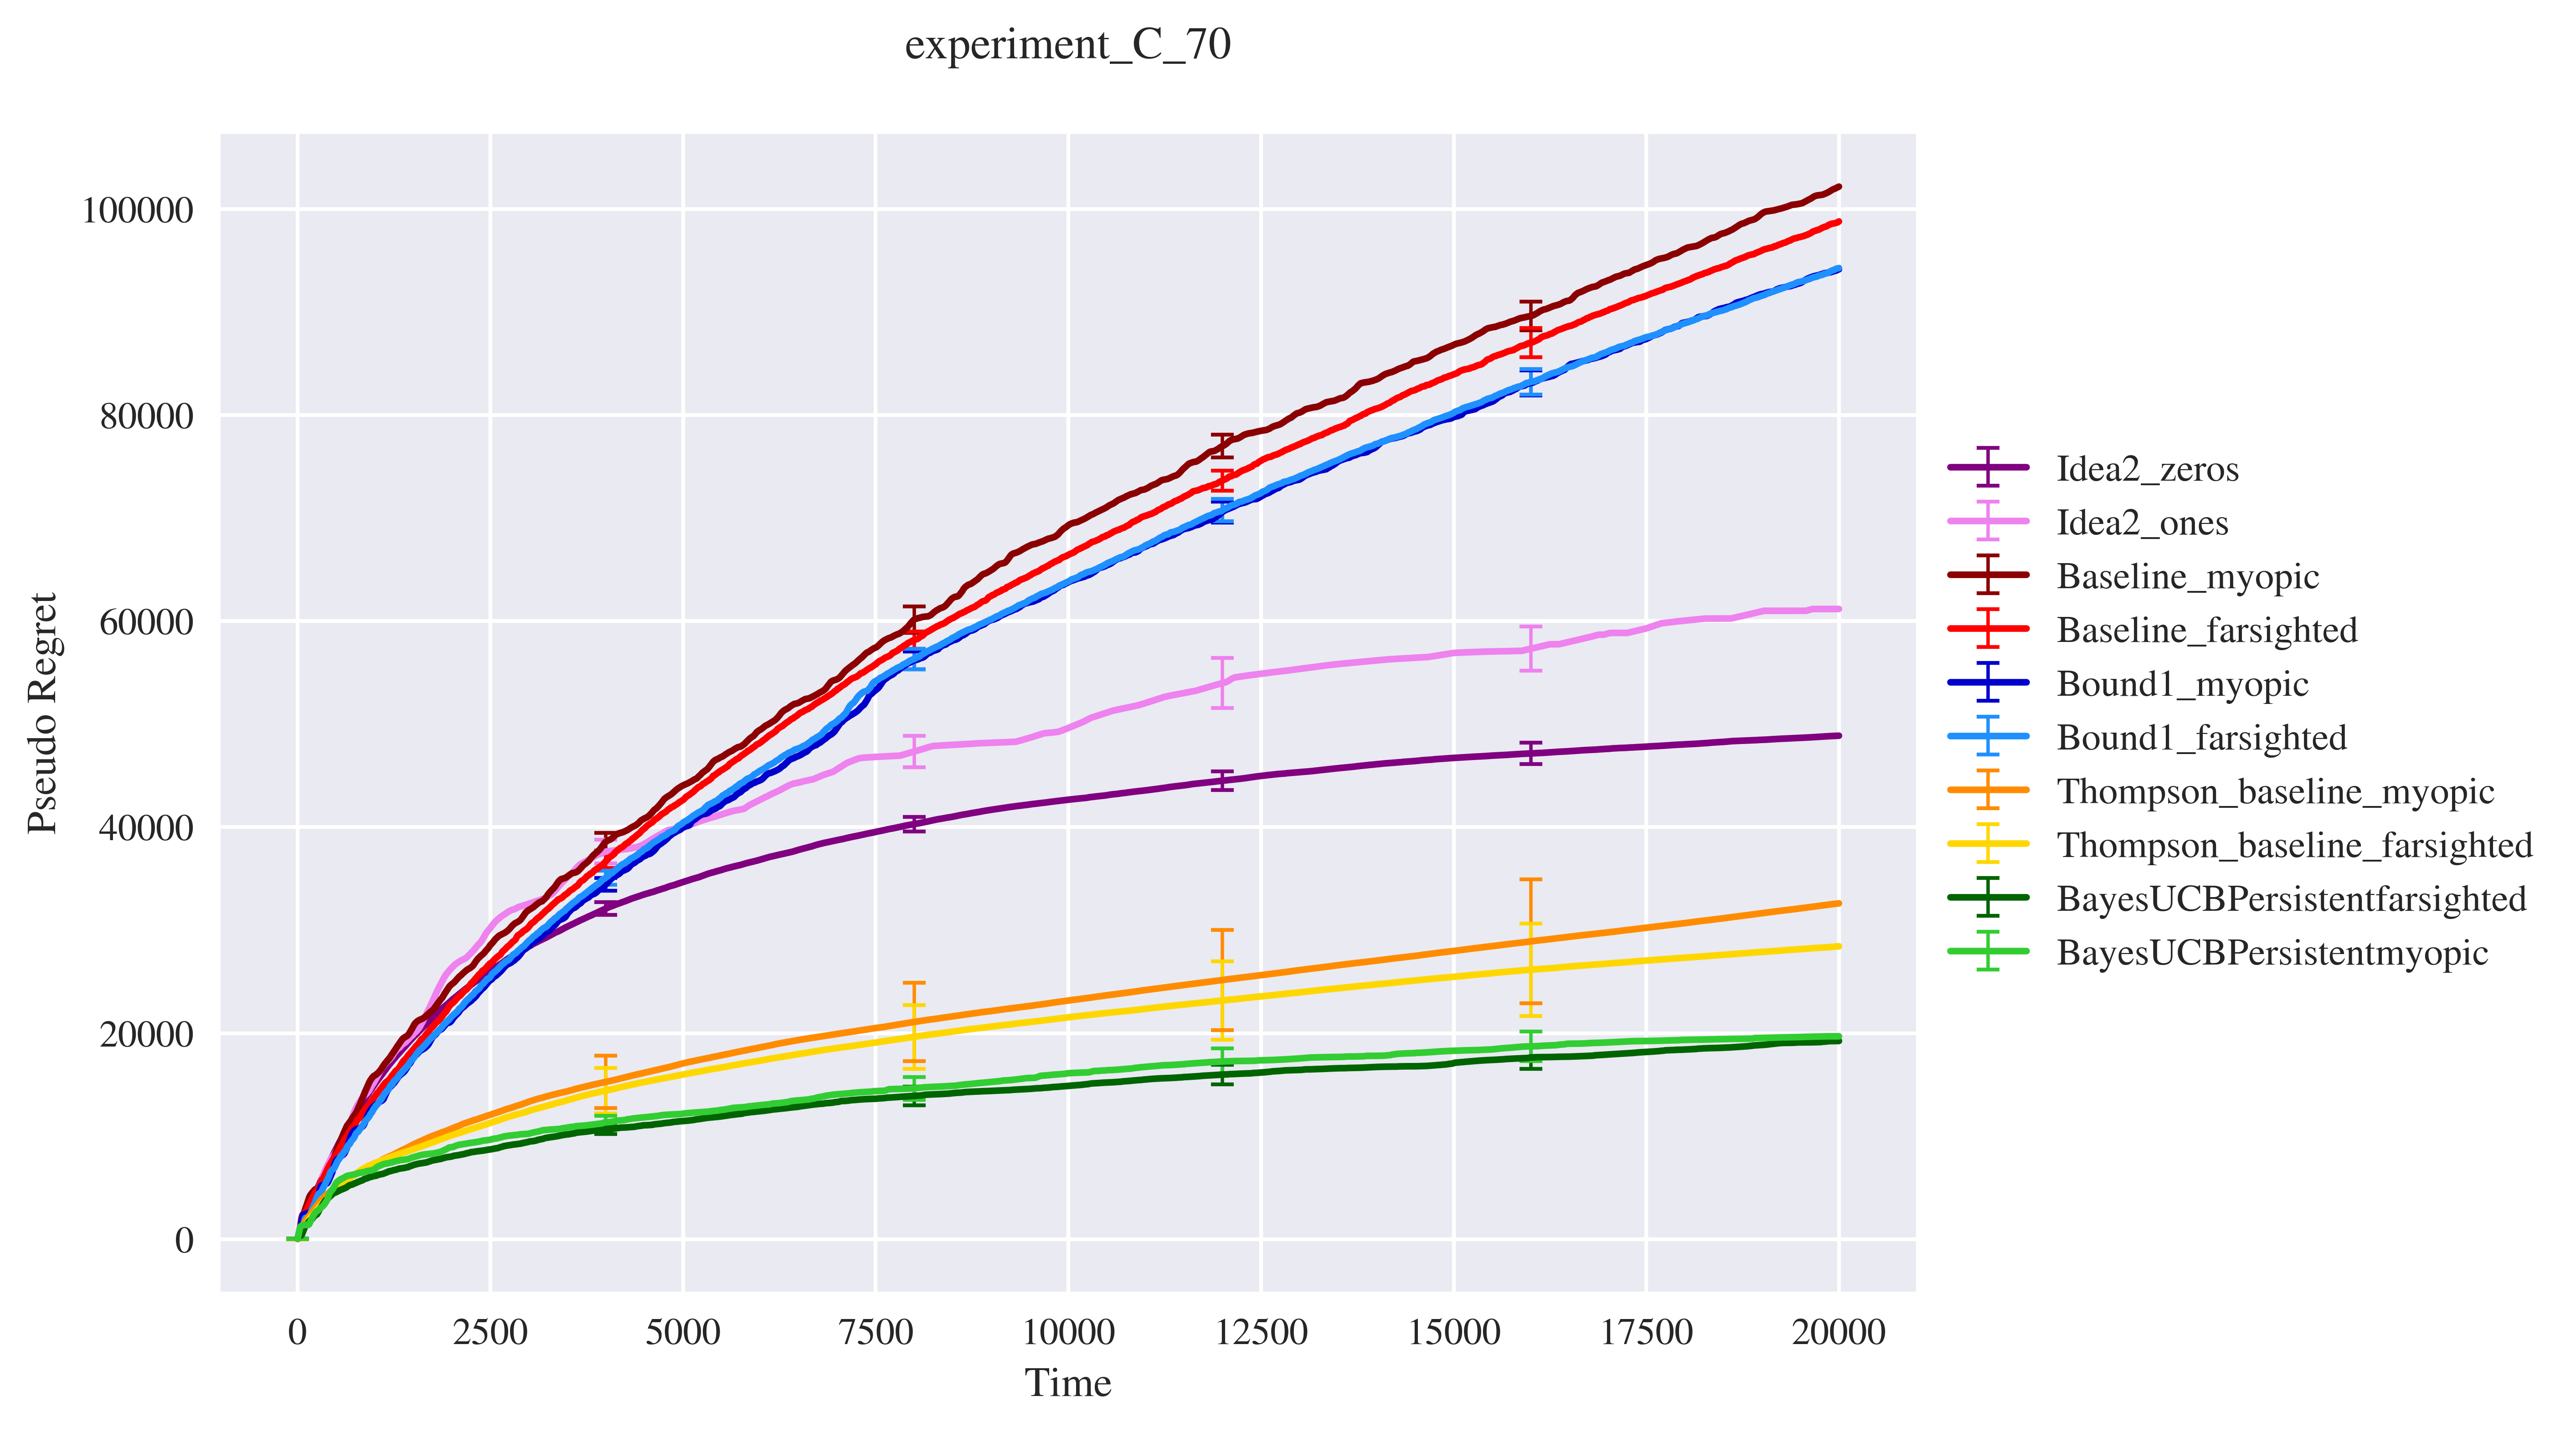
\includegraphics[width=6cm]{./images/C/experiment_C_70 ANALYTICS.png}\quad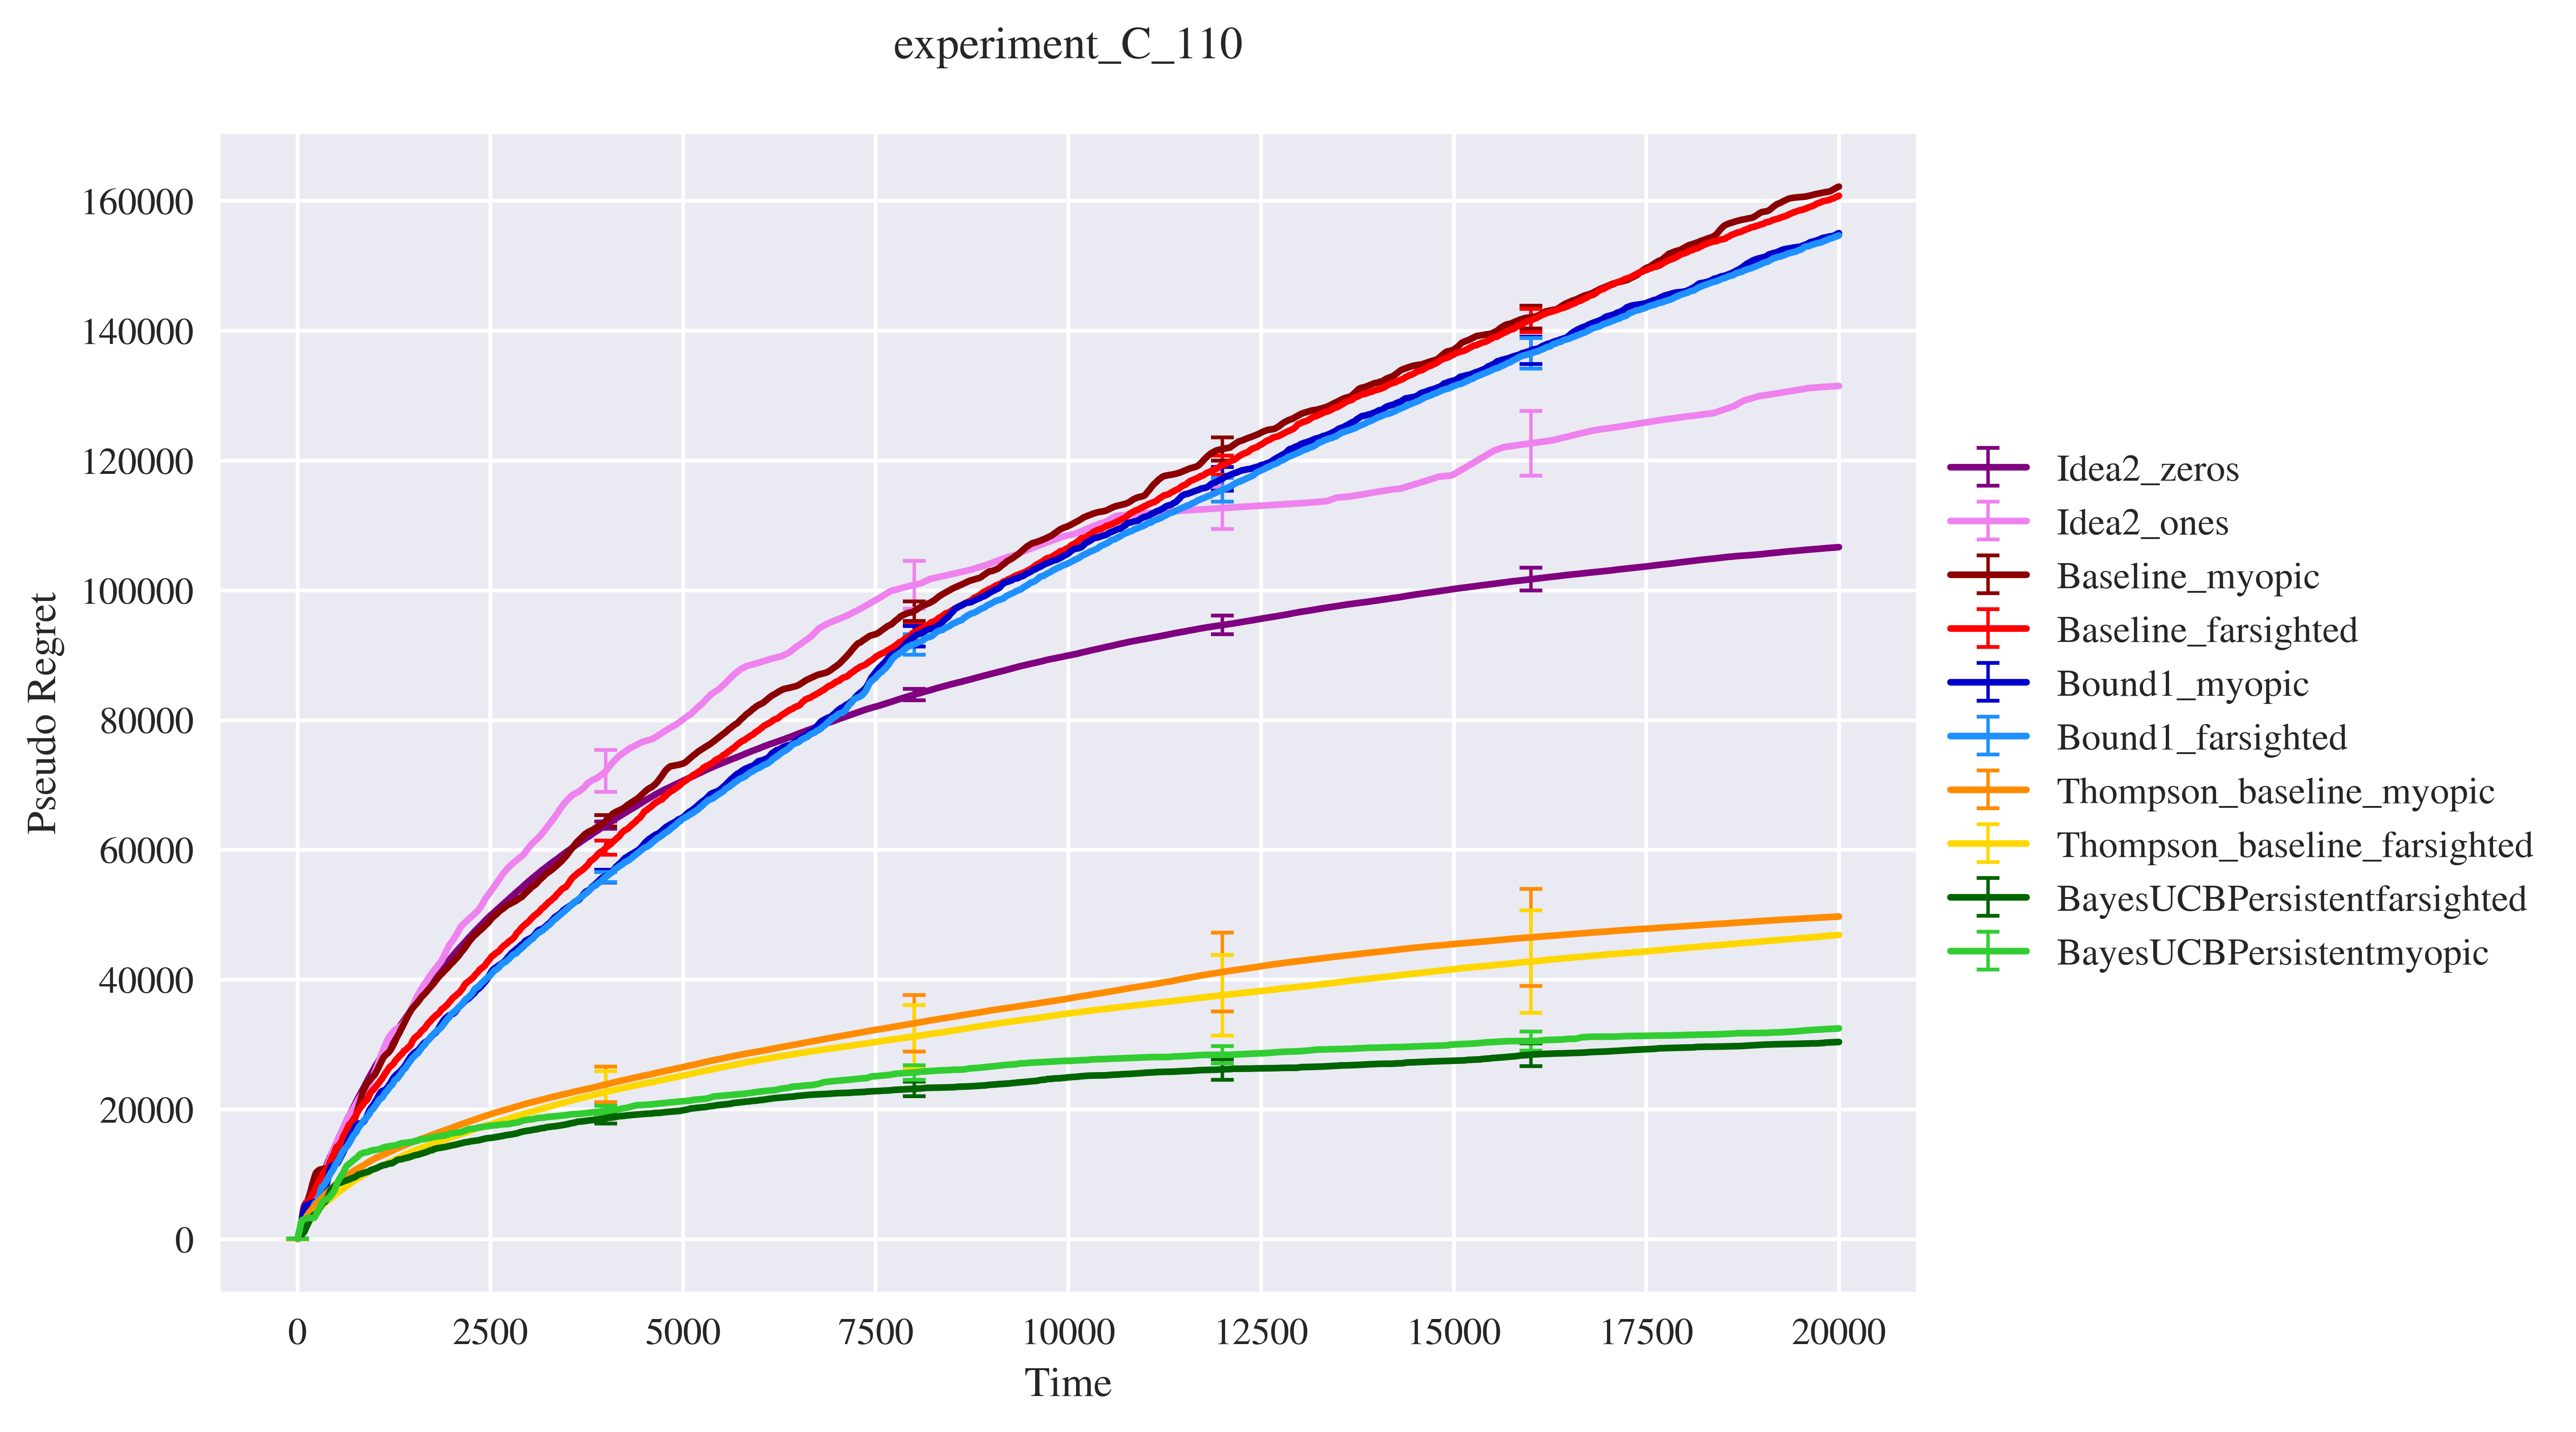
\includegraphics[width=6cm]{./images/C/experiment_C_110 ANALYTICS.png}
	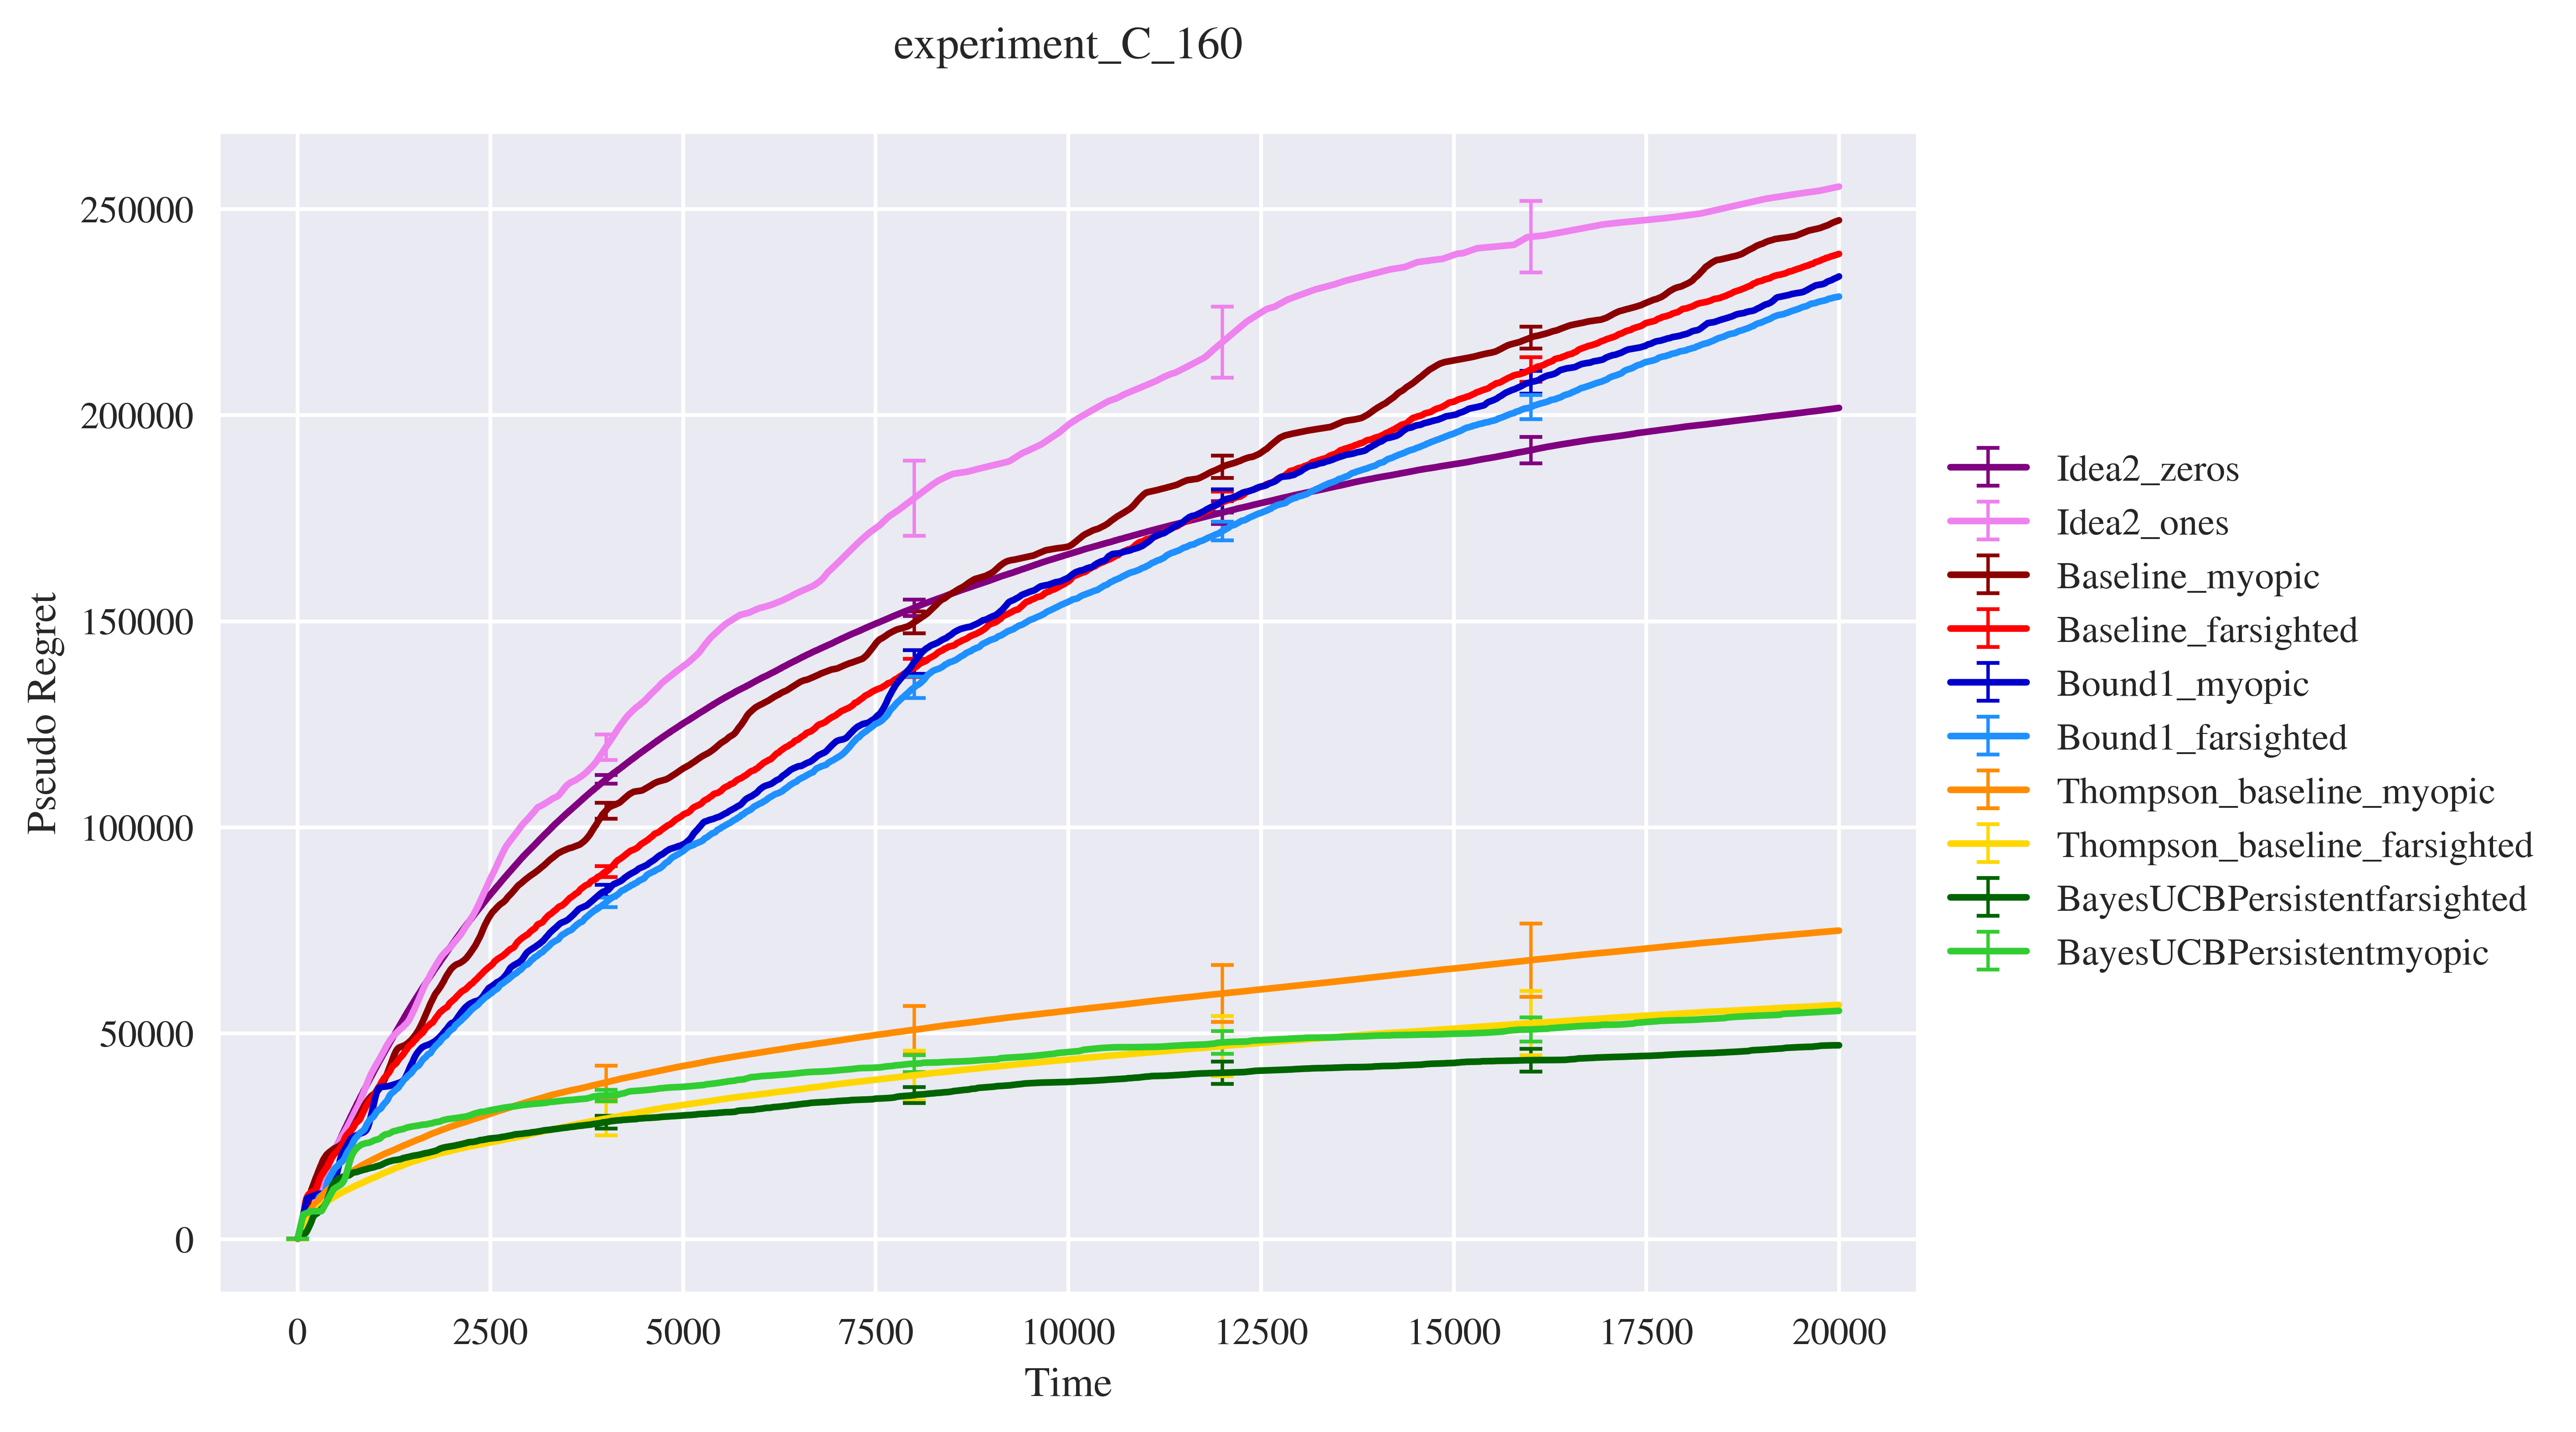
\includegraphics[width=6cm]{./images/C/experiment_C_160 ANALYTICS.png}\quad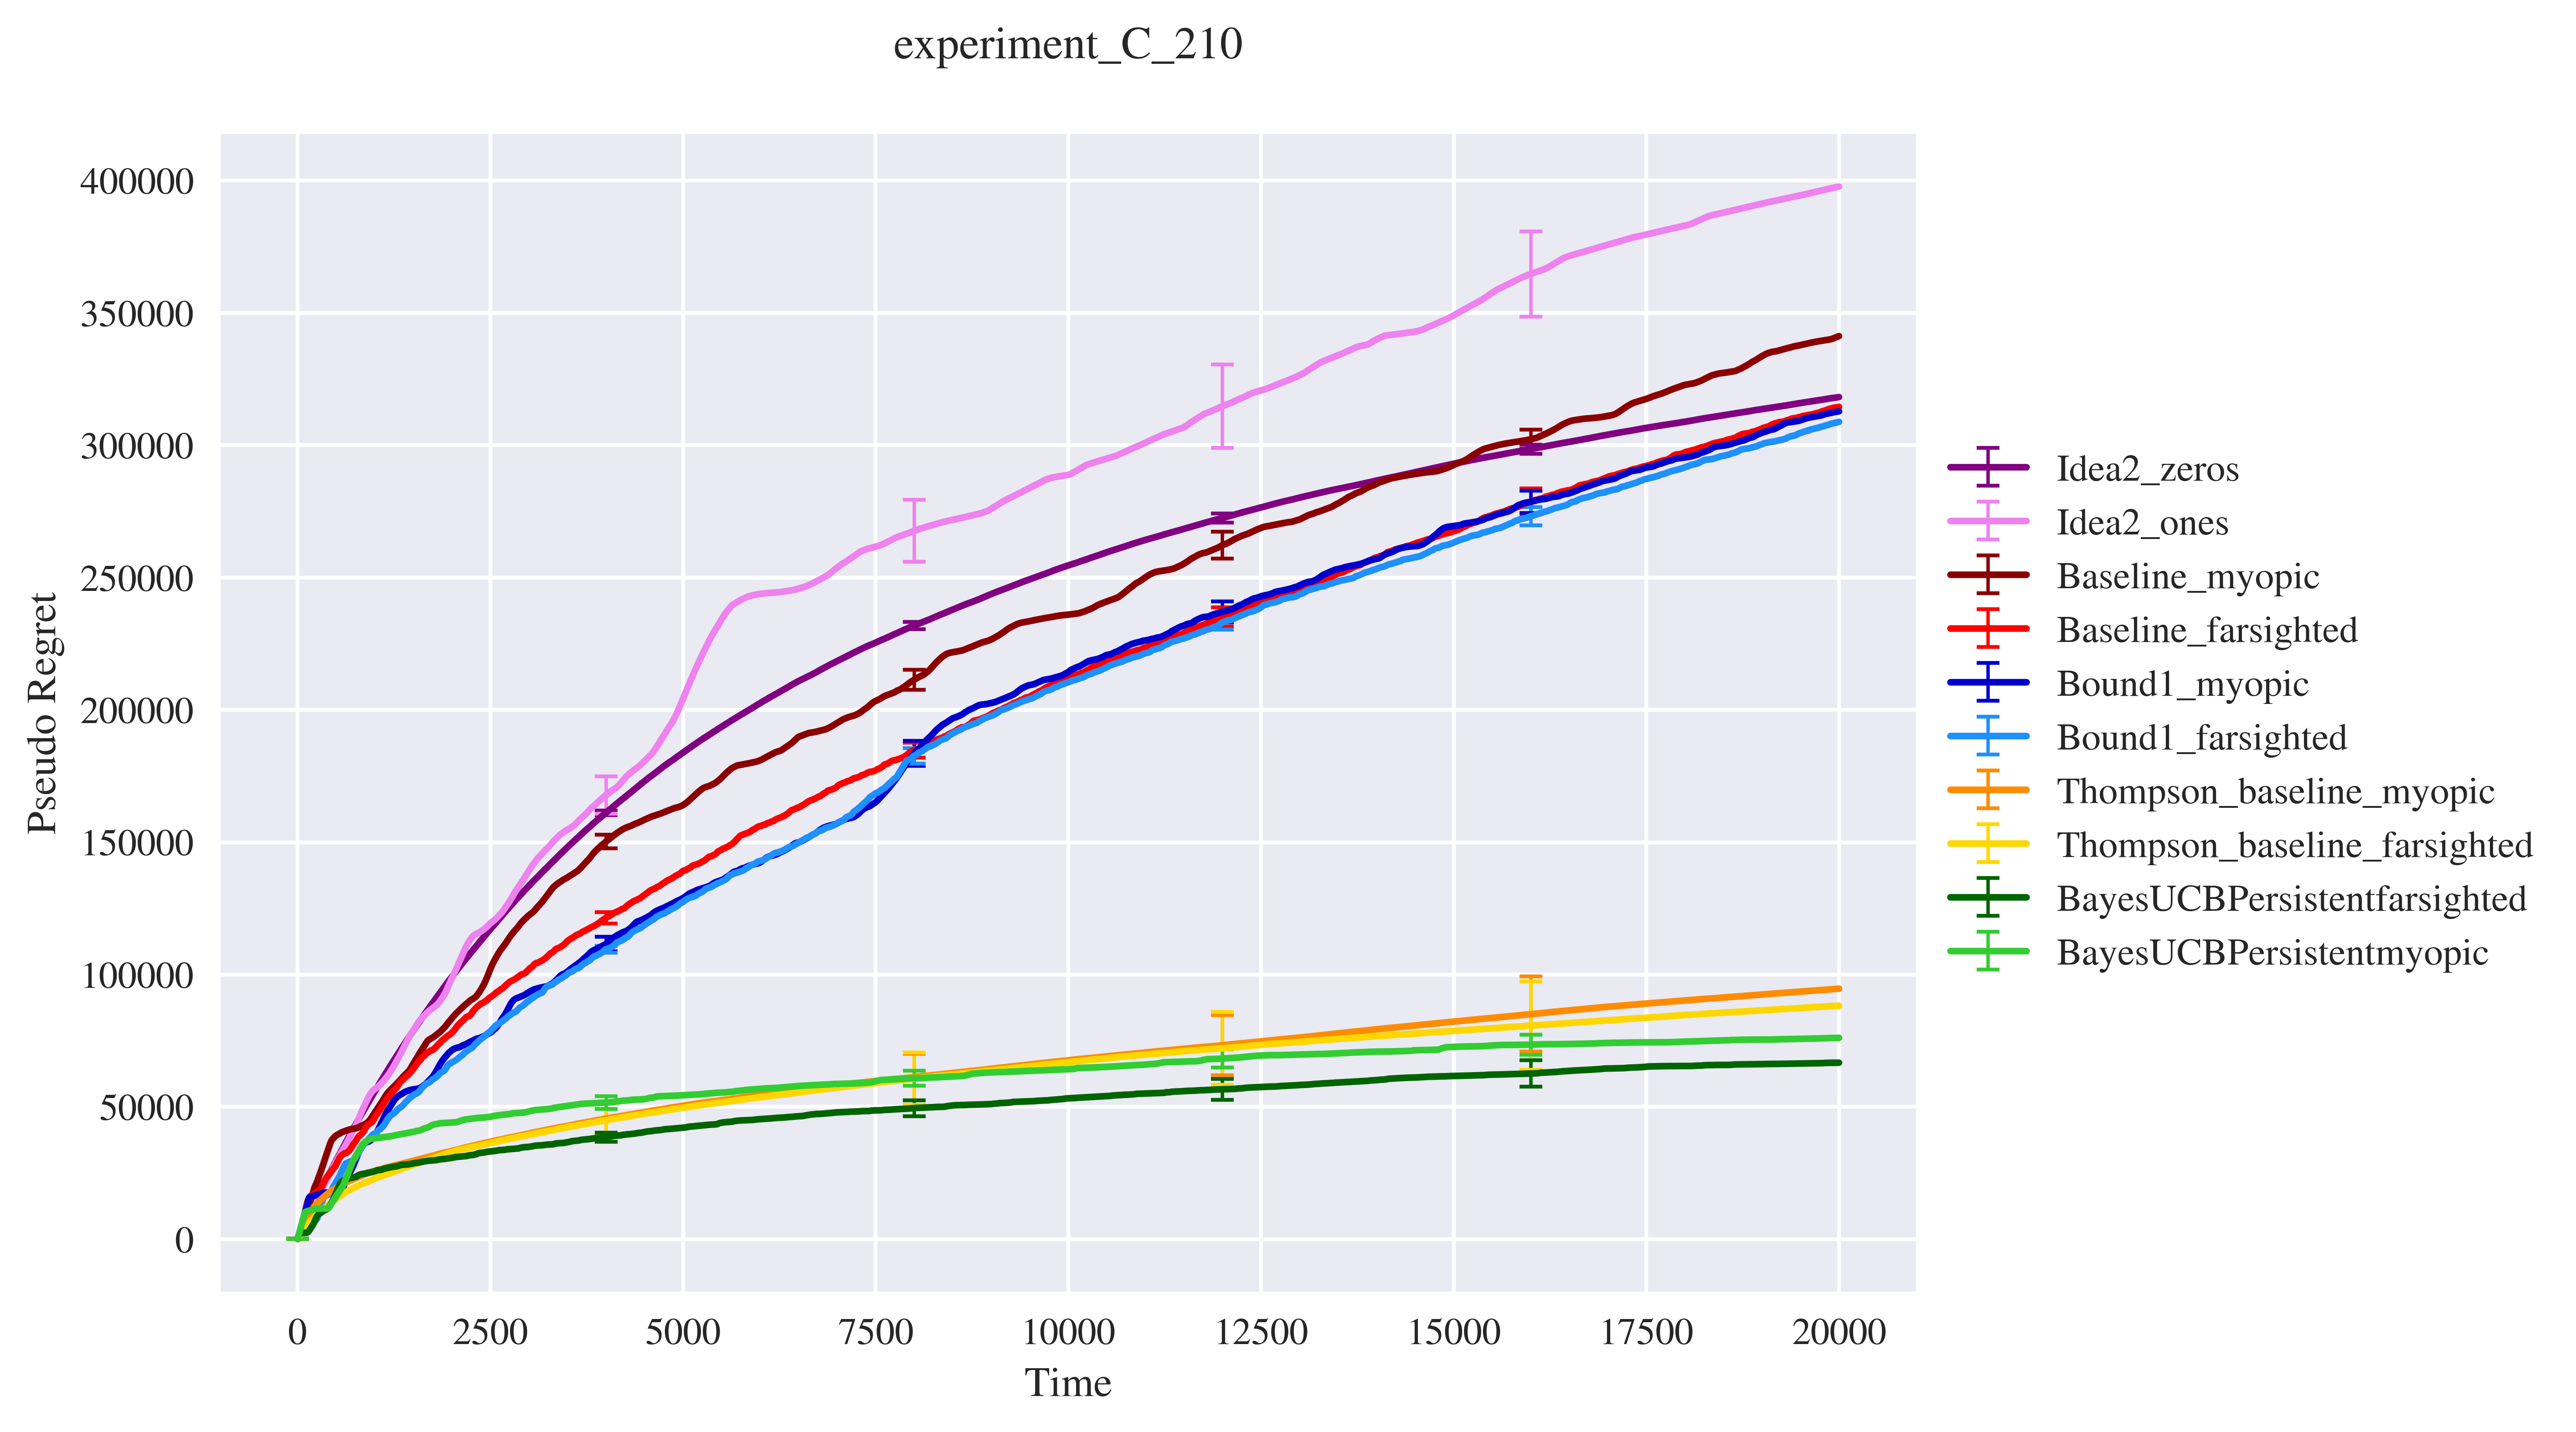
\includegraphics[width=6cm]{./images/C/experiment_C_210 ANALYTICS.png}
	\caption{SYNTHETIC C}
	
\end{figure}



\begin{figure}[h]
	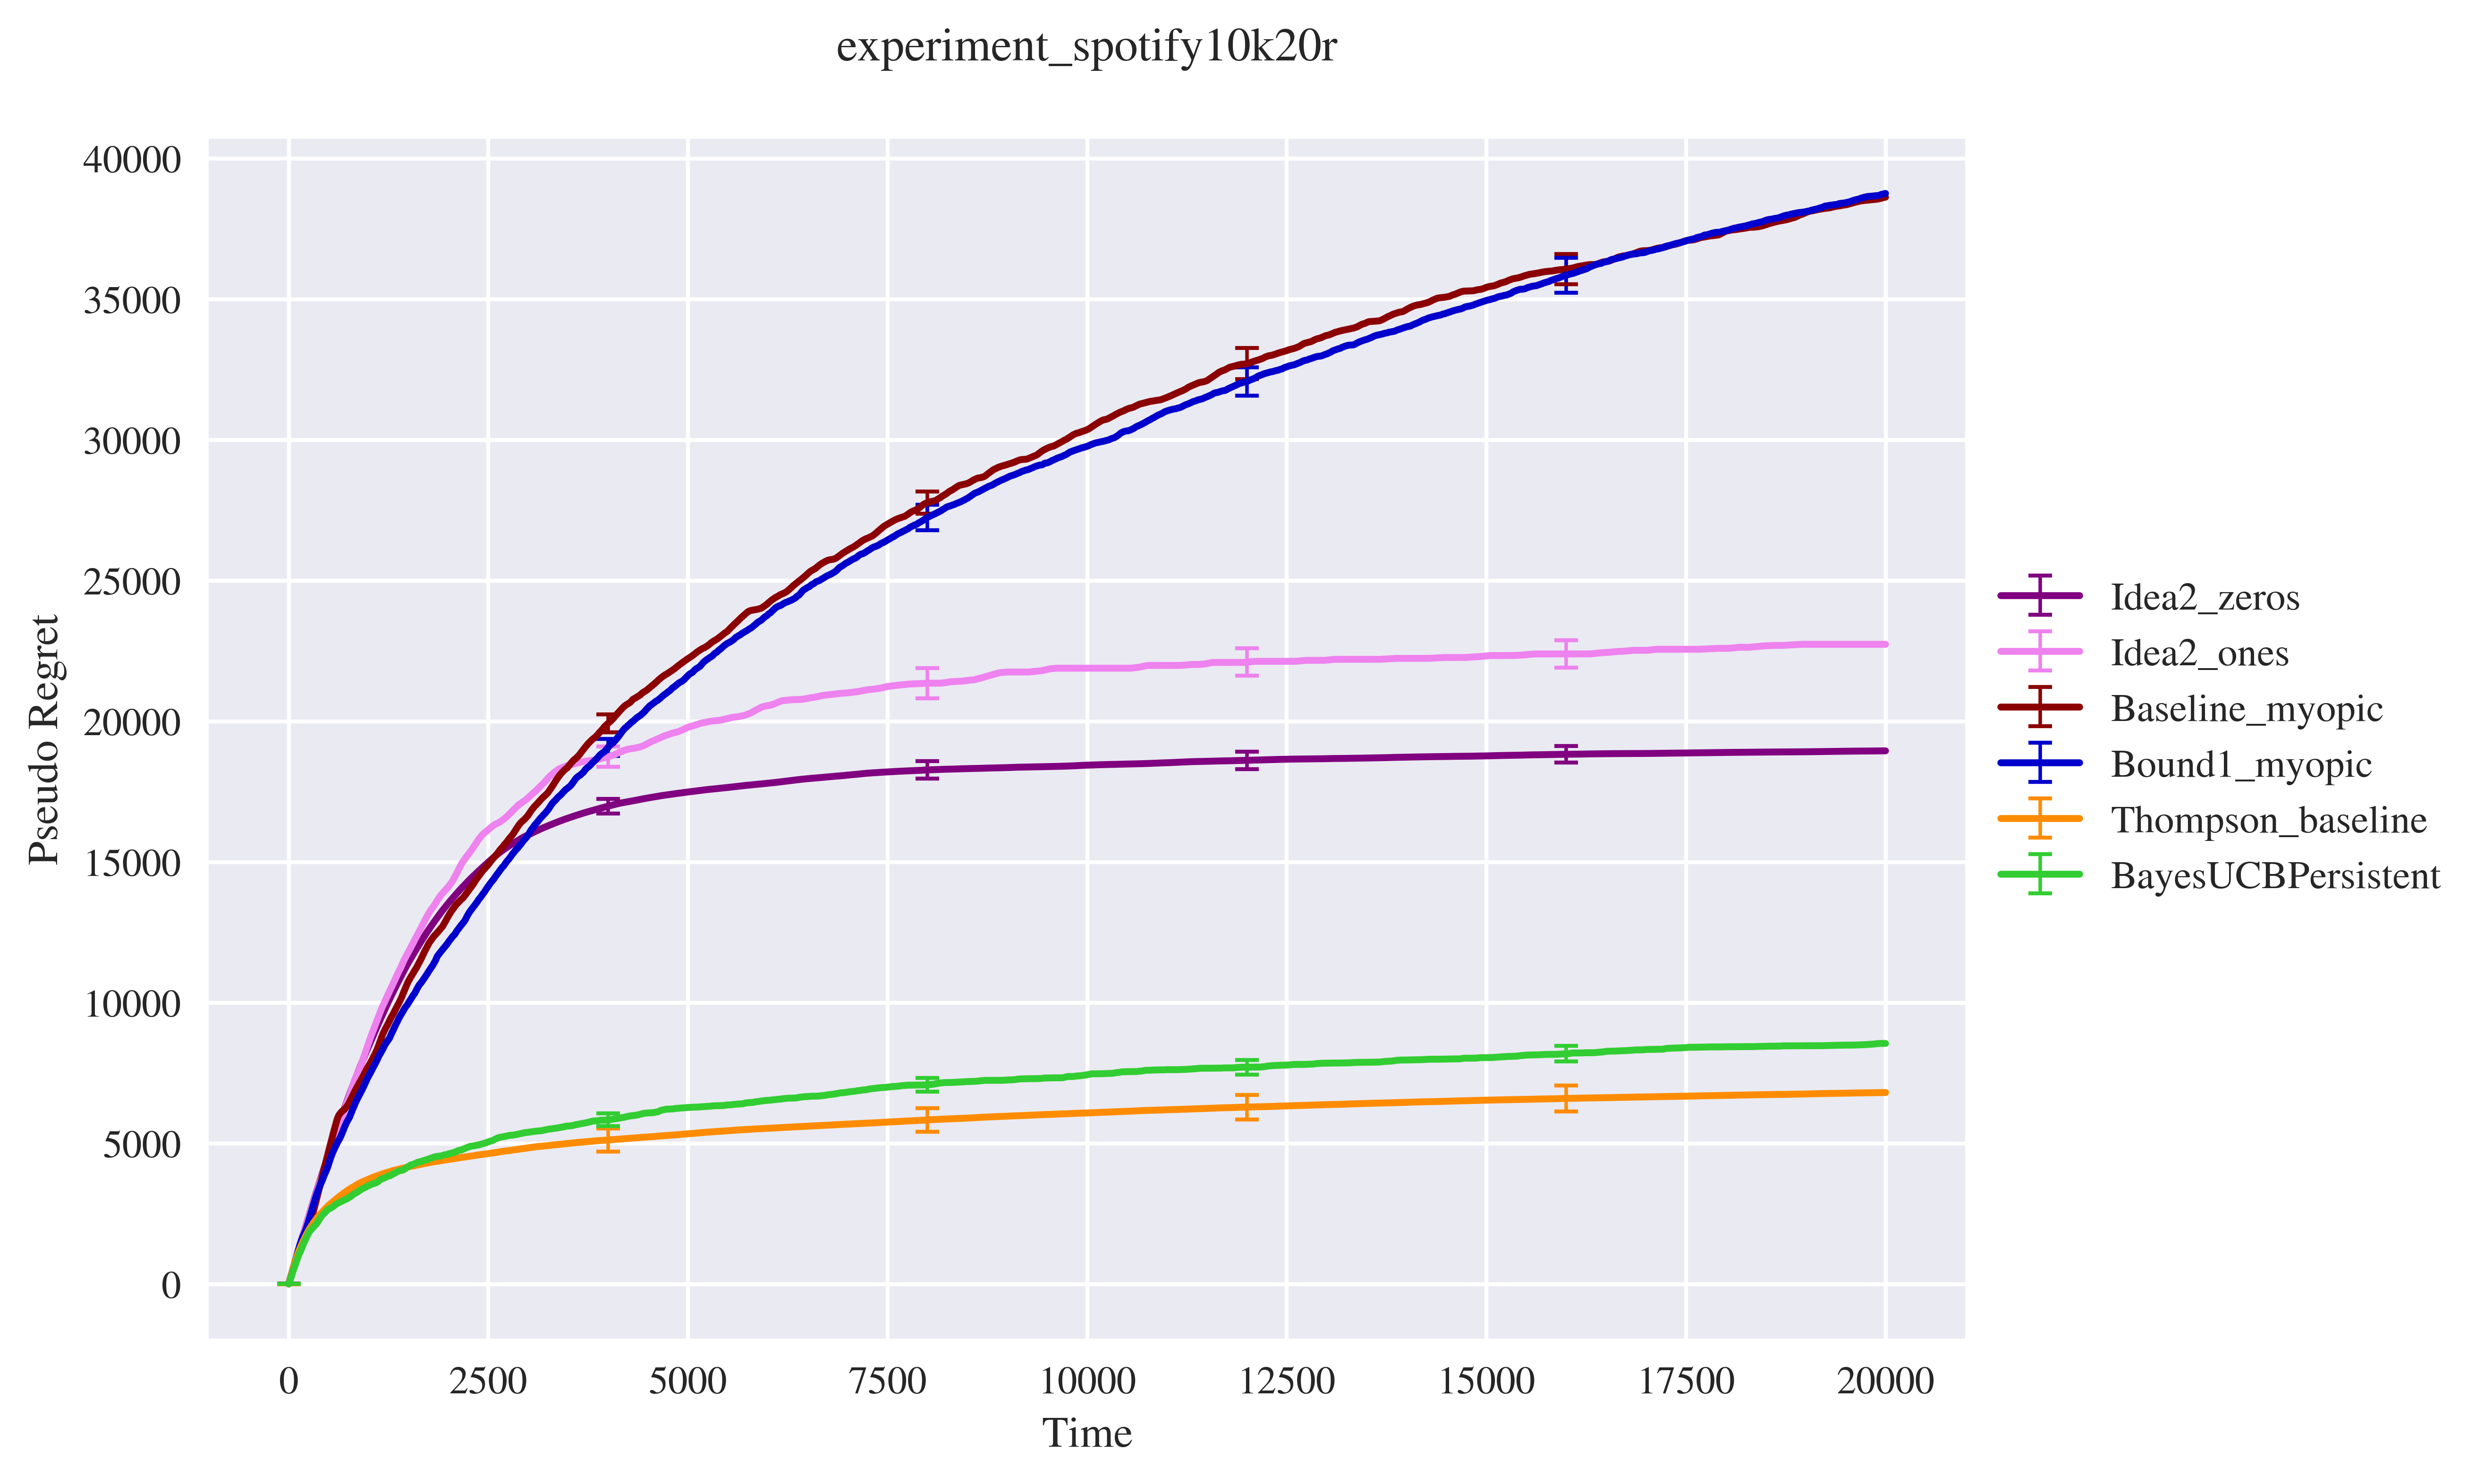
\includegraphics[width=16cm]{./images/experiment_spotify10k20r ANALYTICS.png}
	\centering	
	\caption{Spotify Scenario}
\end{figure}


\begin{figure}
	\centering
	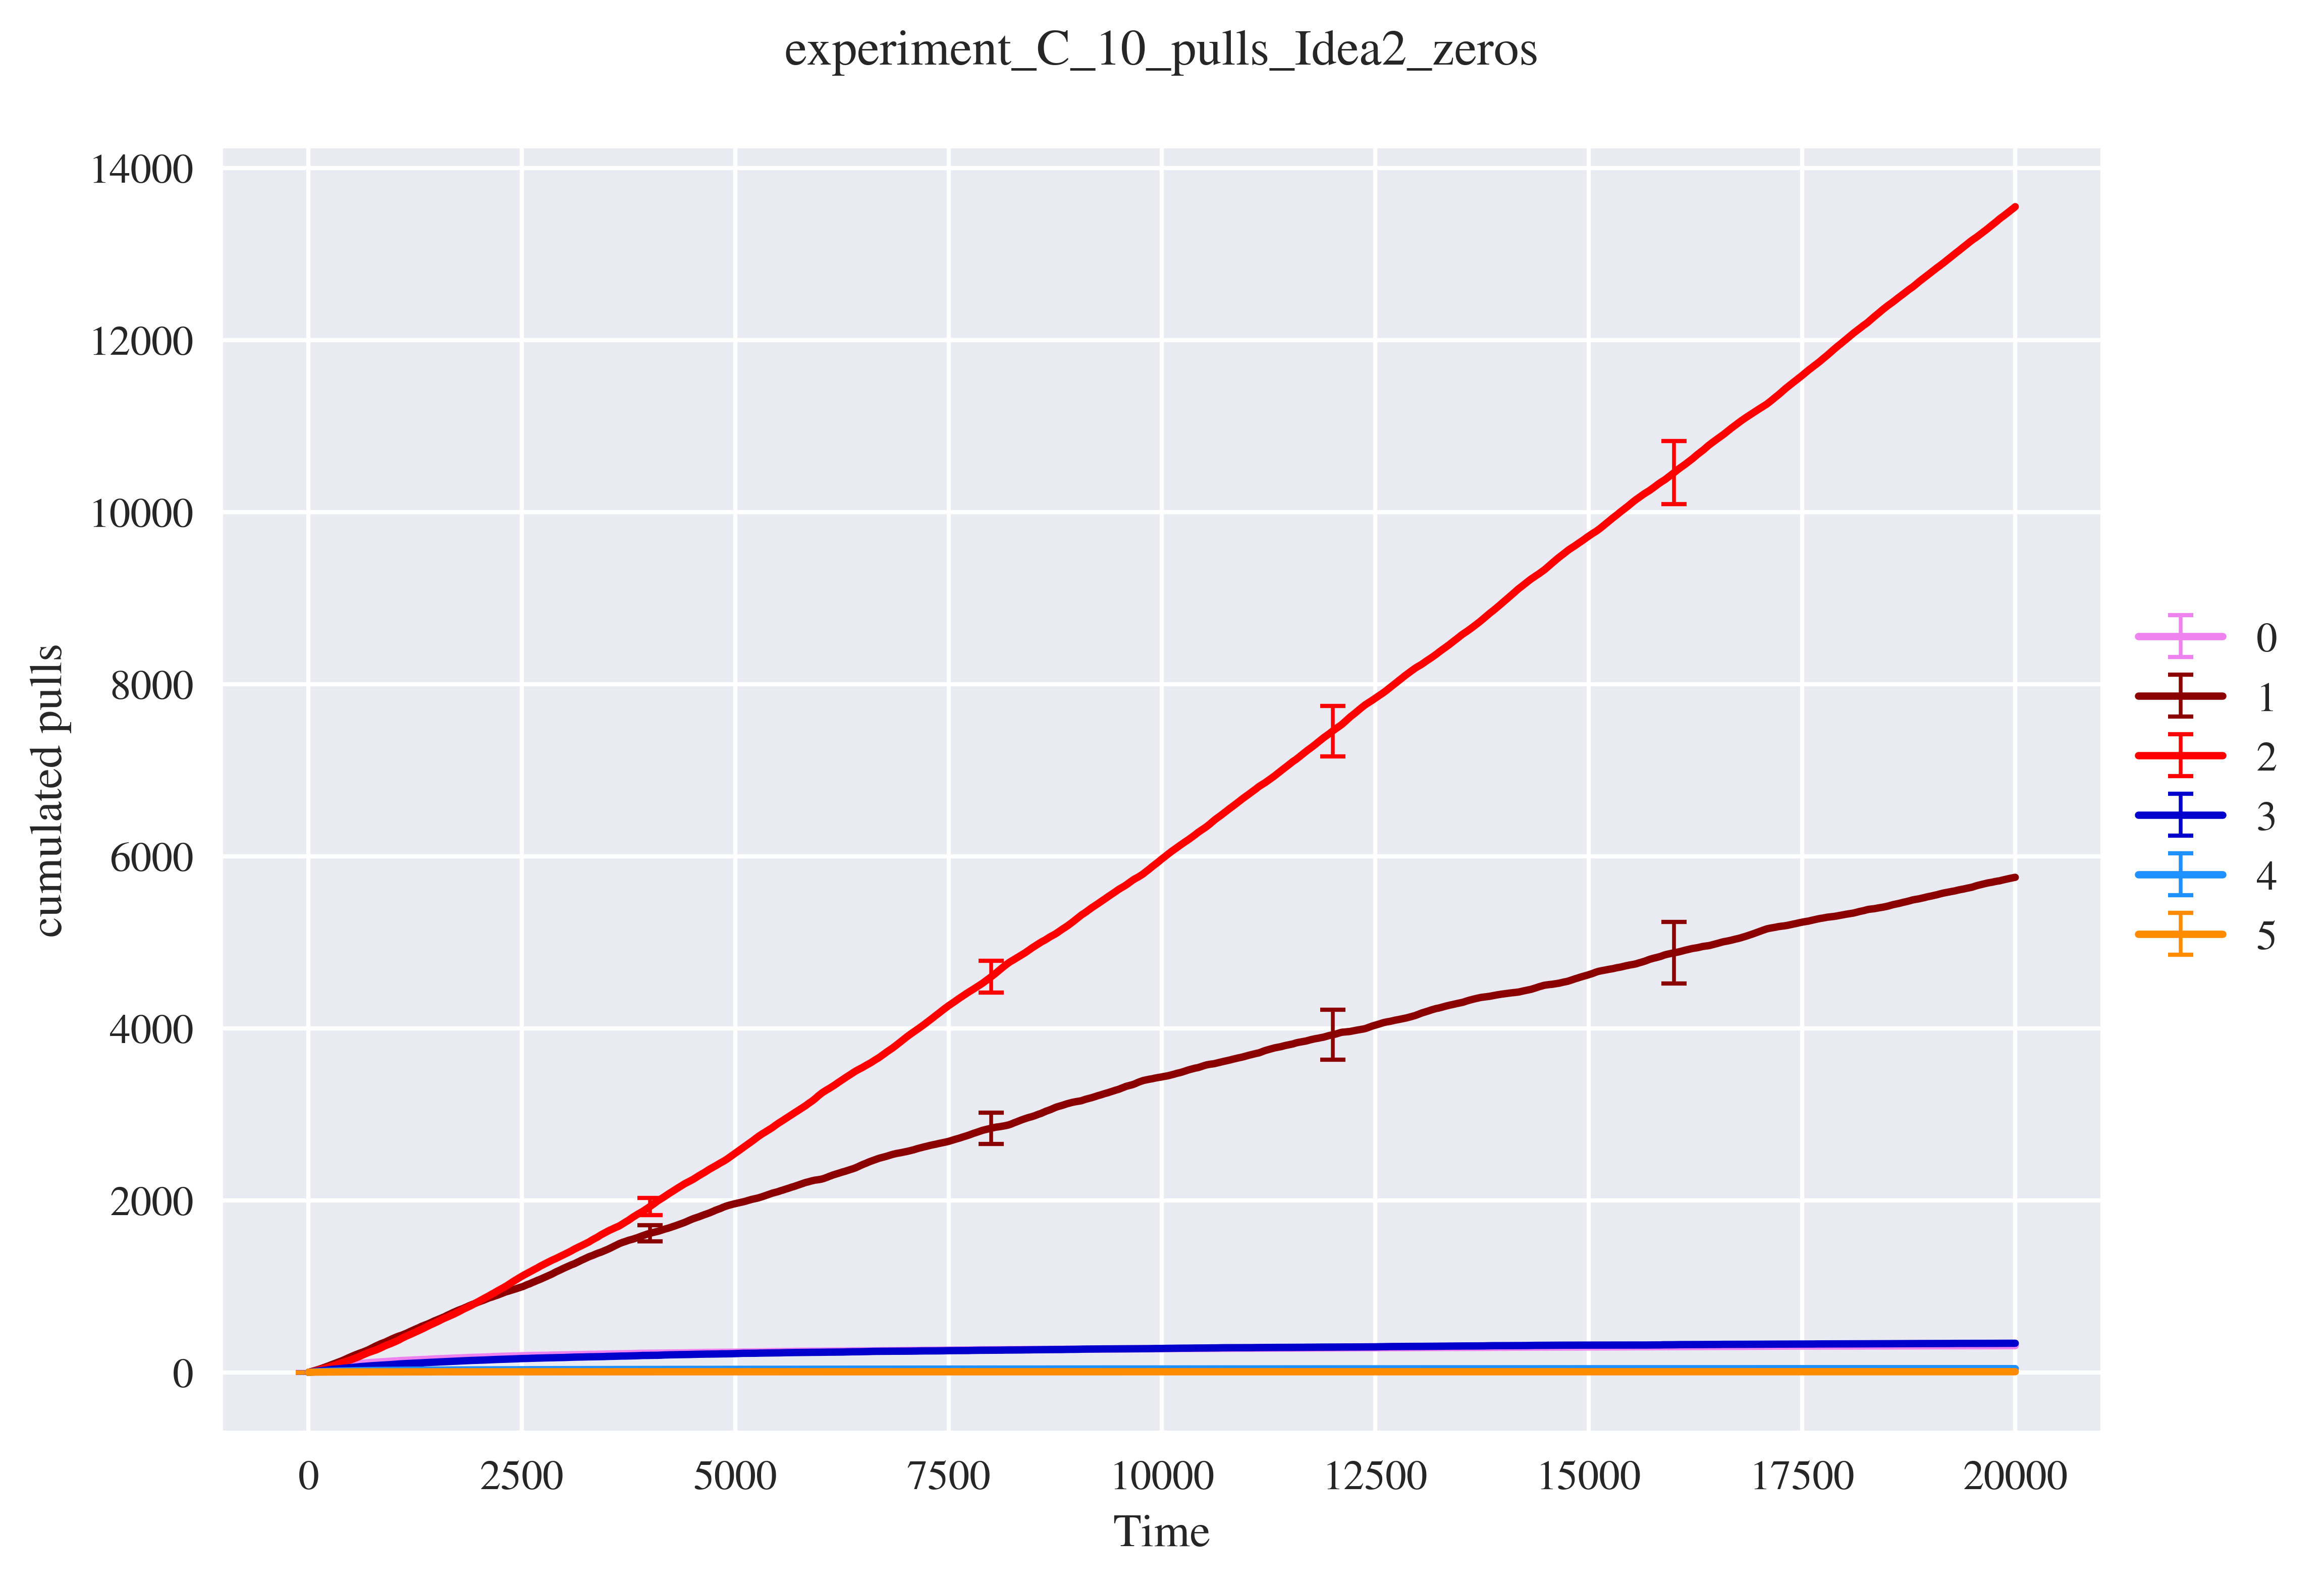
\includegraphics[width=6cm]{./images/PULLS/experiment_C_10Idea2_zeros cum_pulls.png }\quad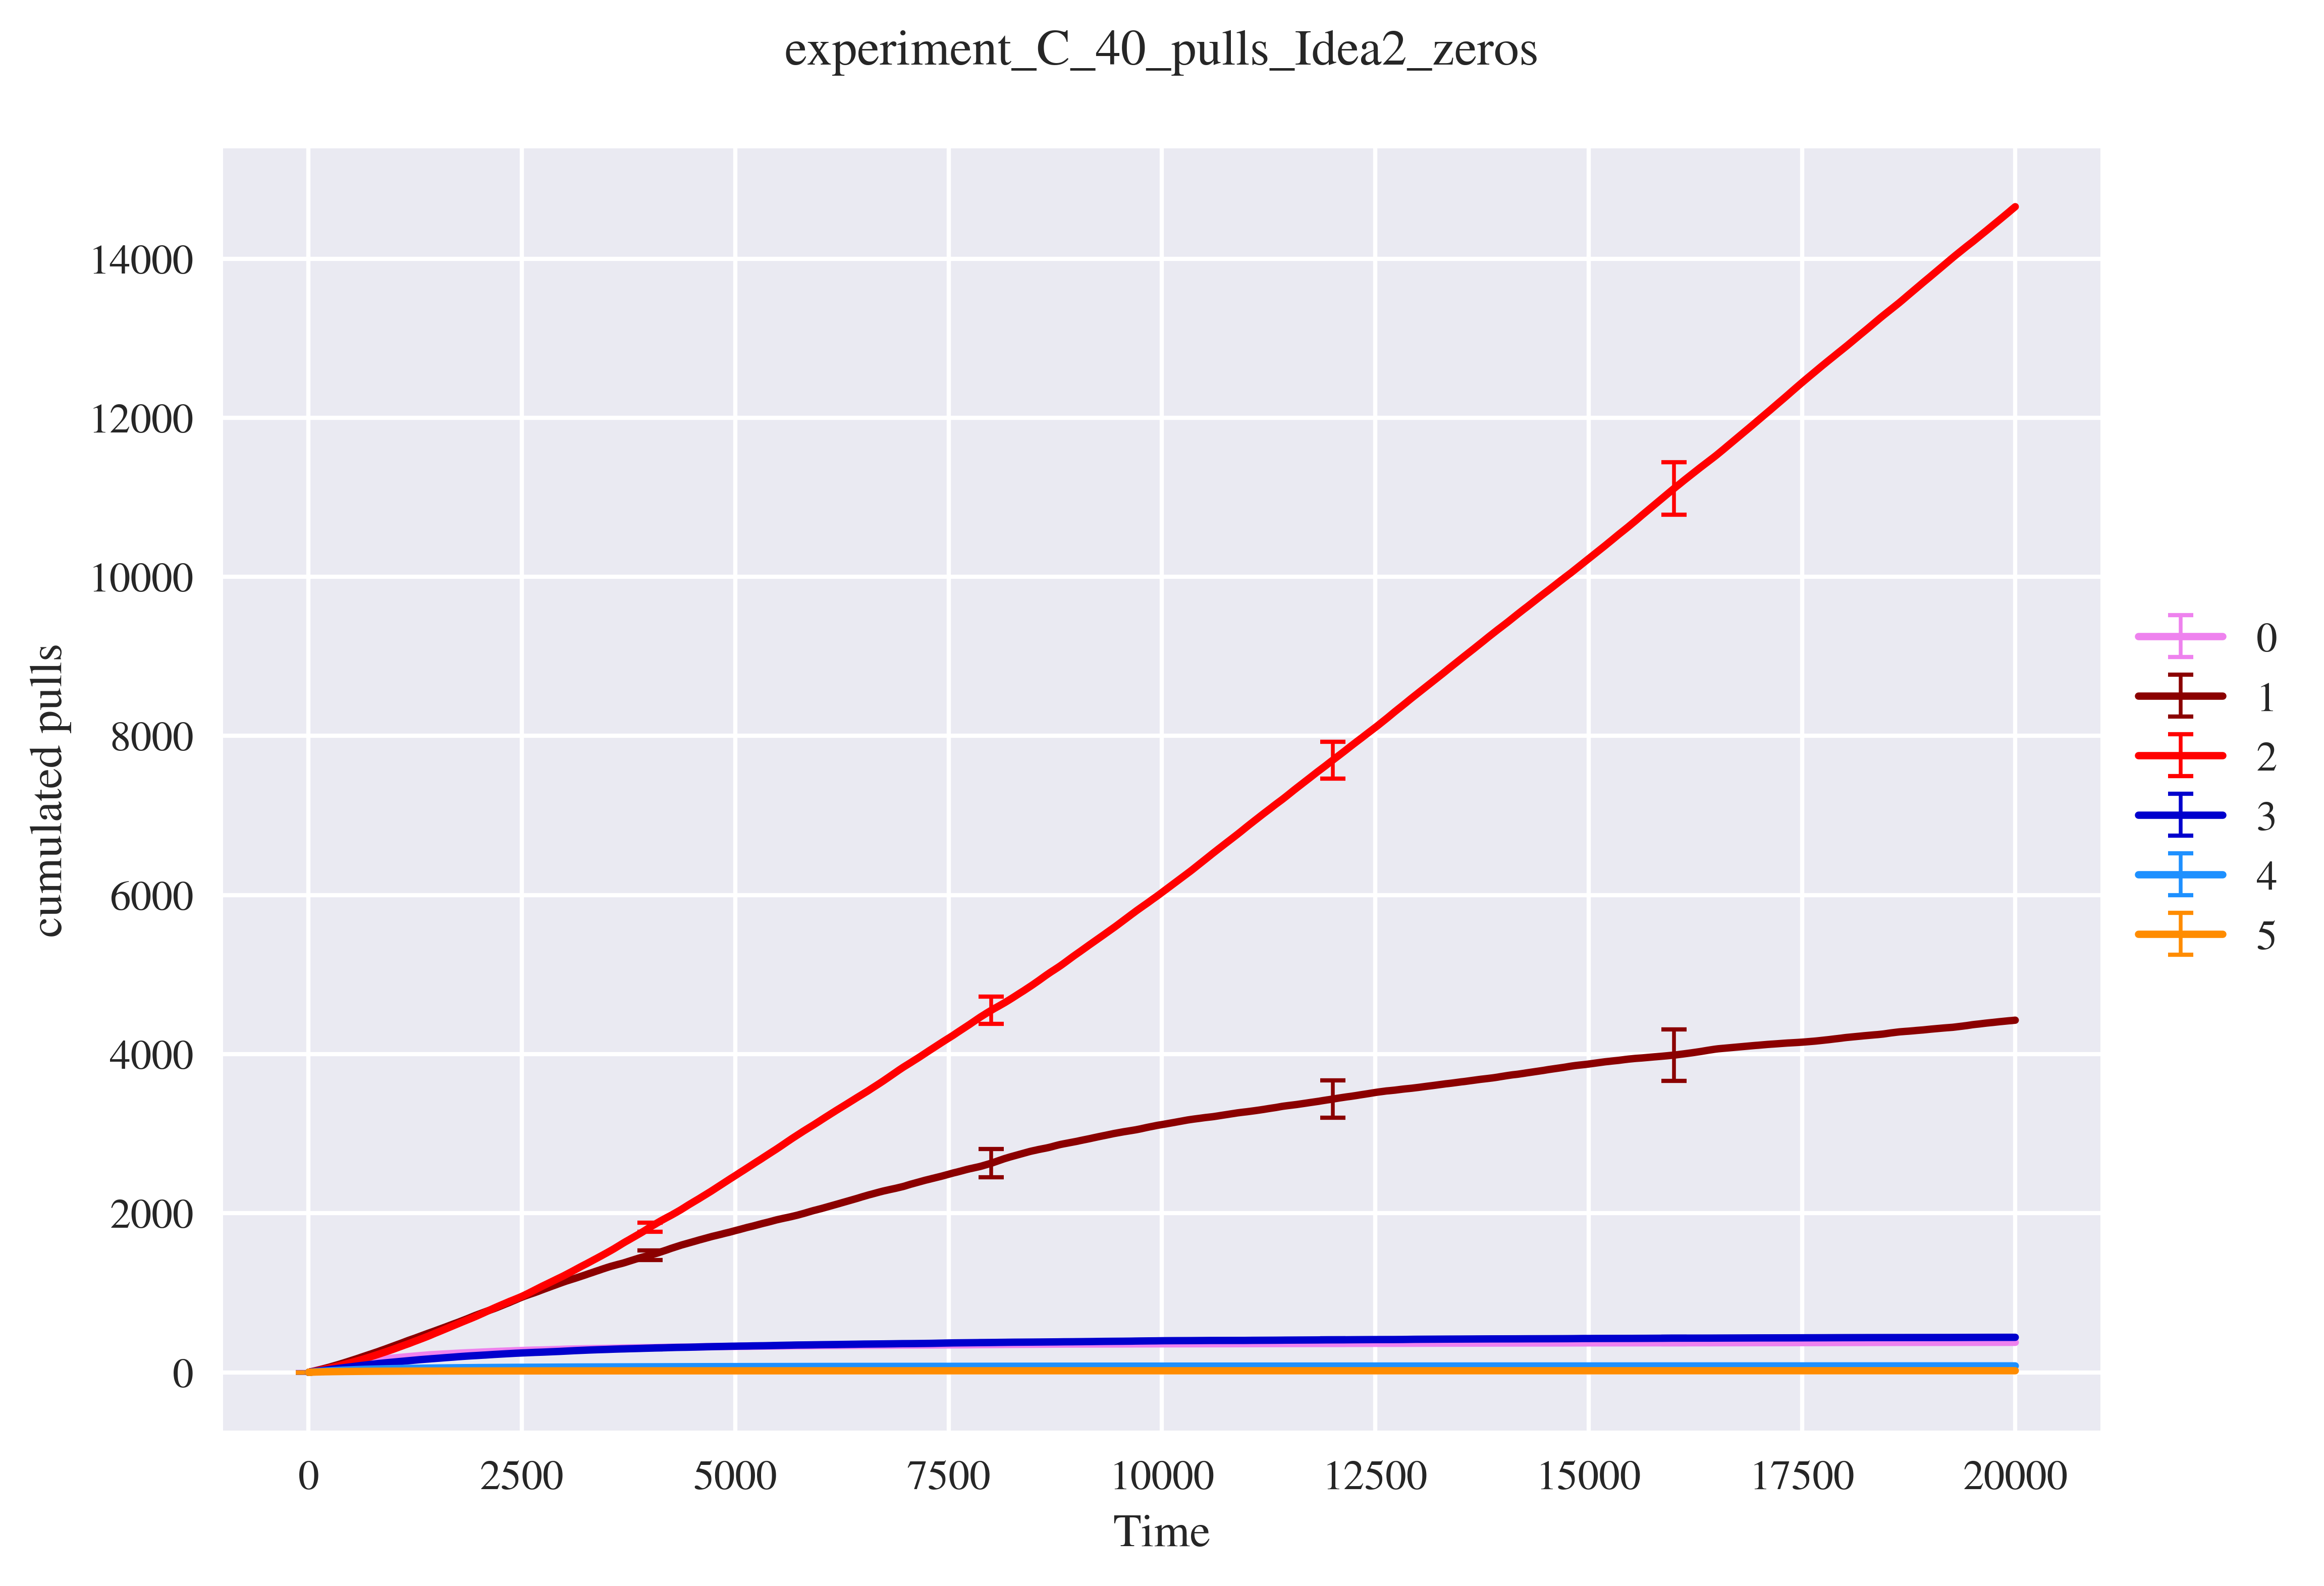
\includegraphics[width=6cm]{./images/PULLS/experiment_C_40Idea2_zeros cum_pulls.png
	} 
	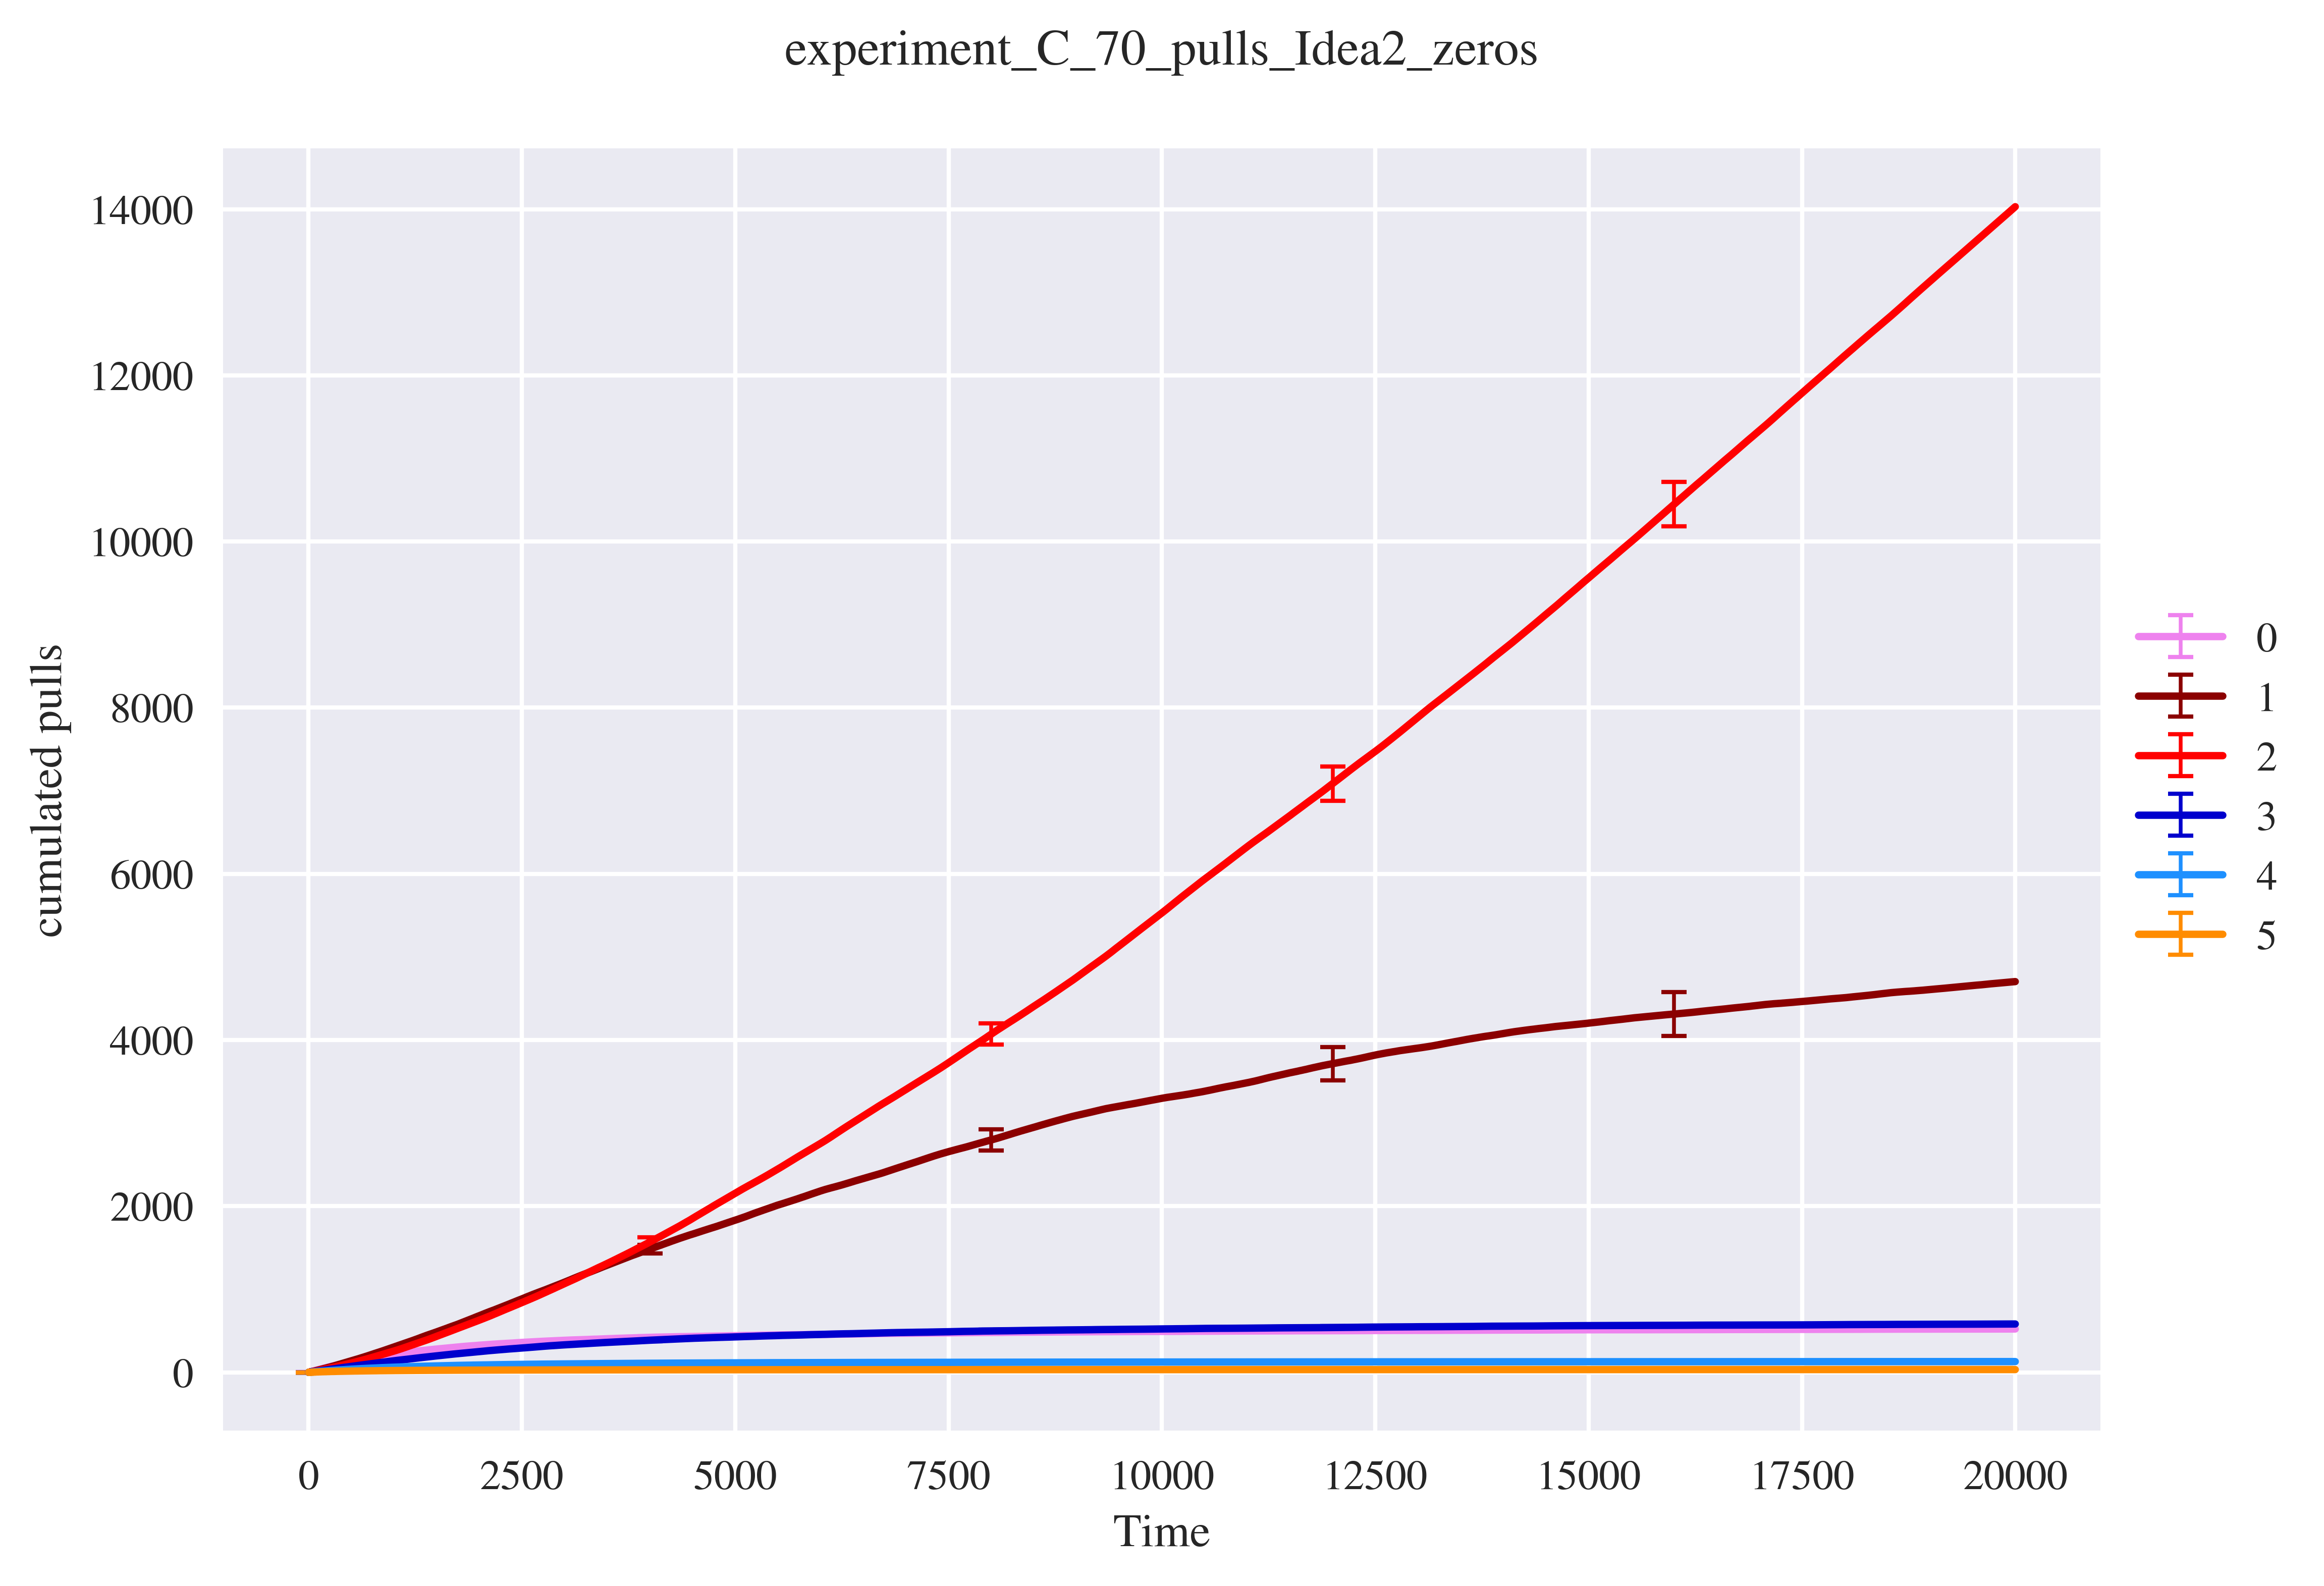
\includegraphics[width=6cm]{./images/PULLS/experiment_C_70Idea2_zeros cum_pulls.png}\quad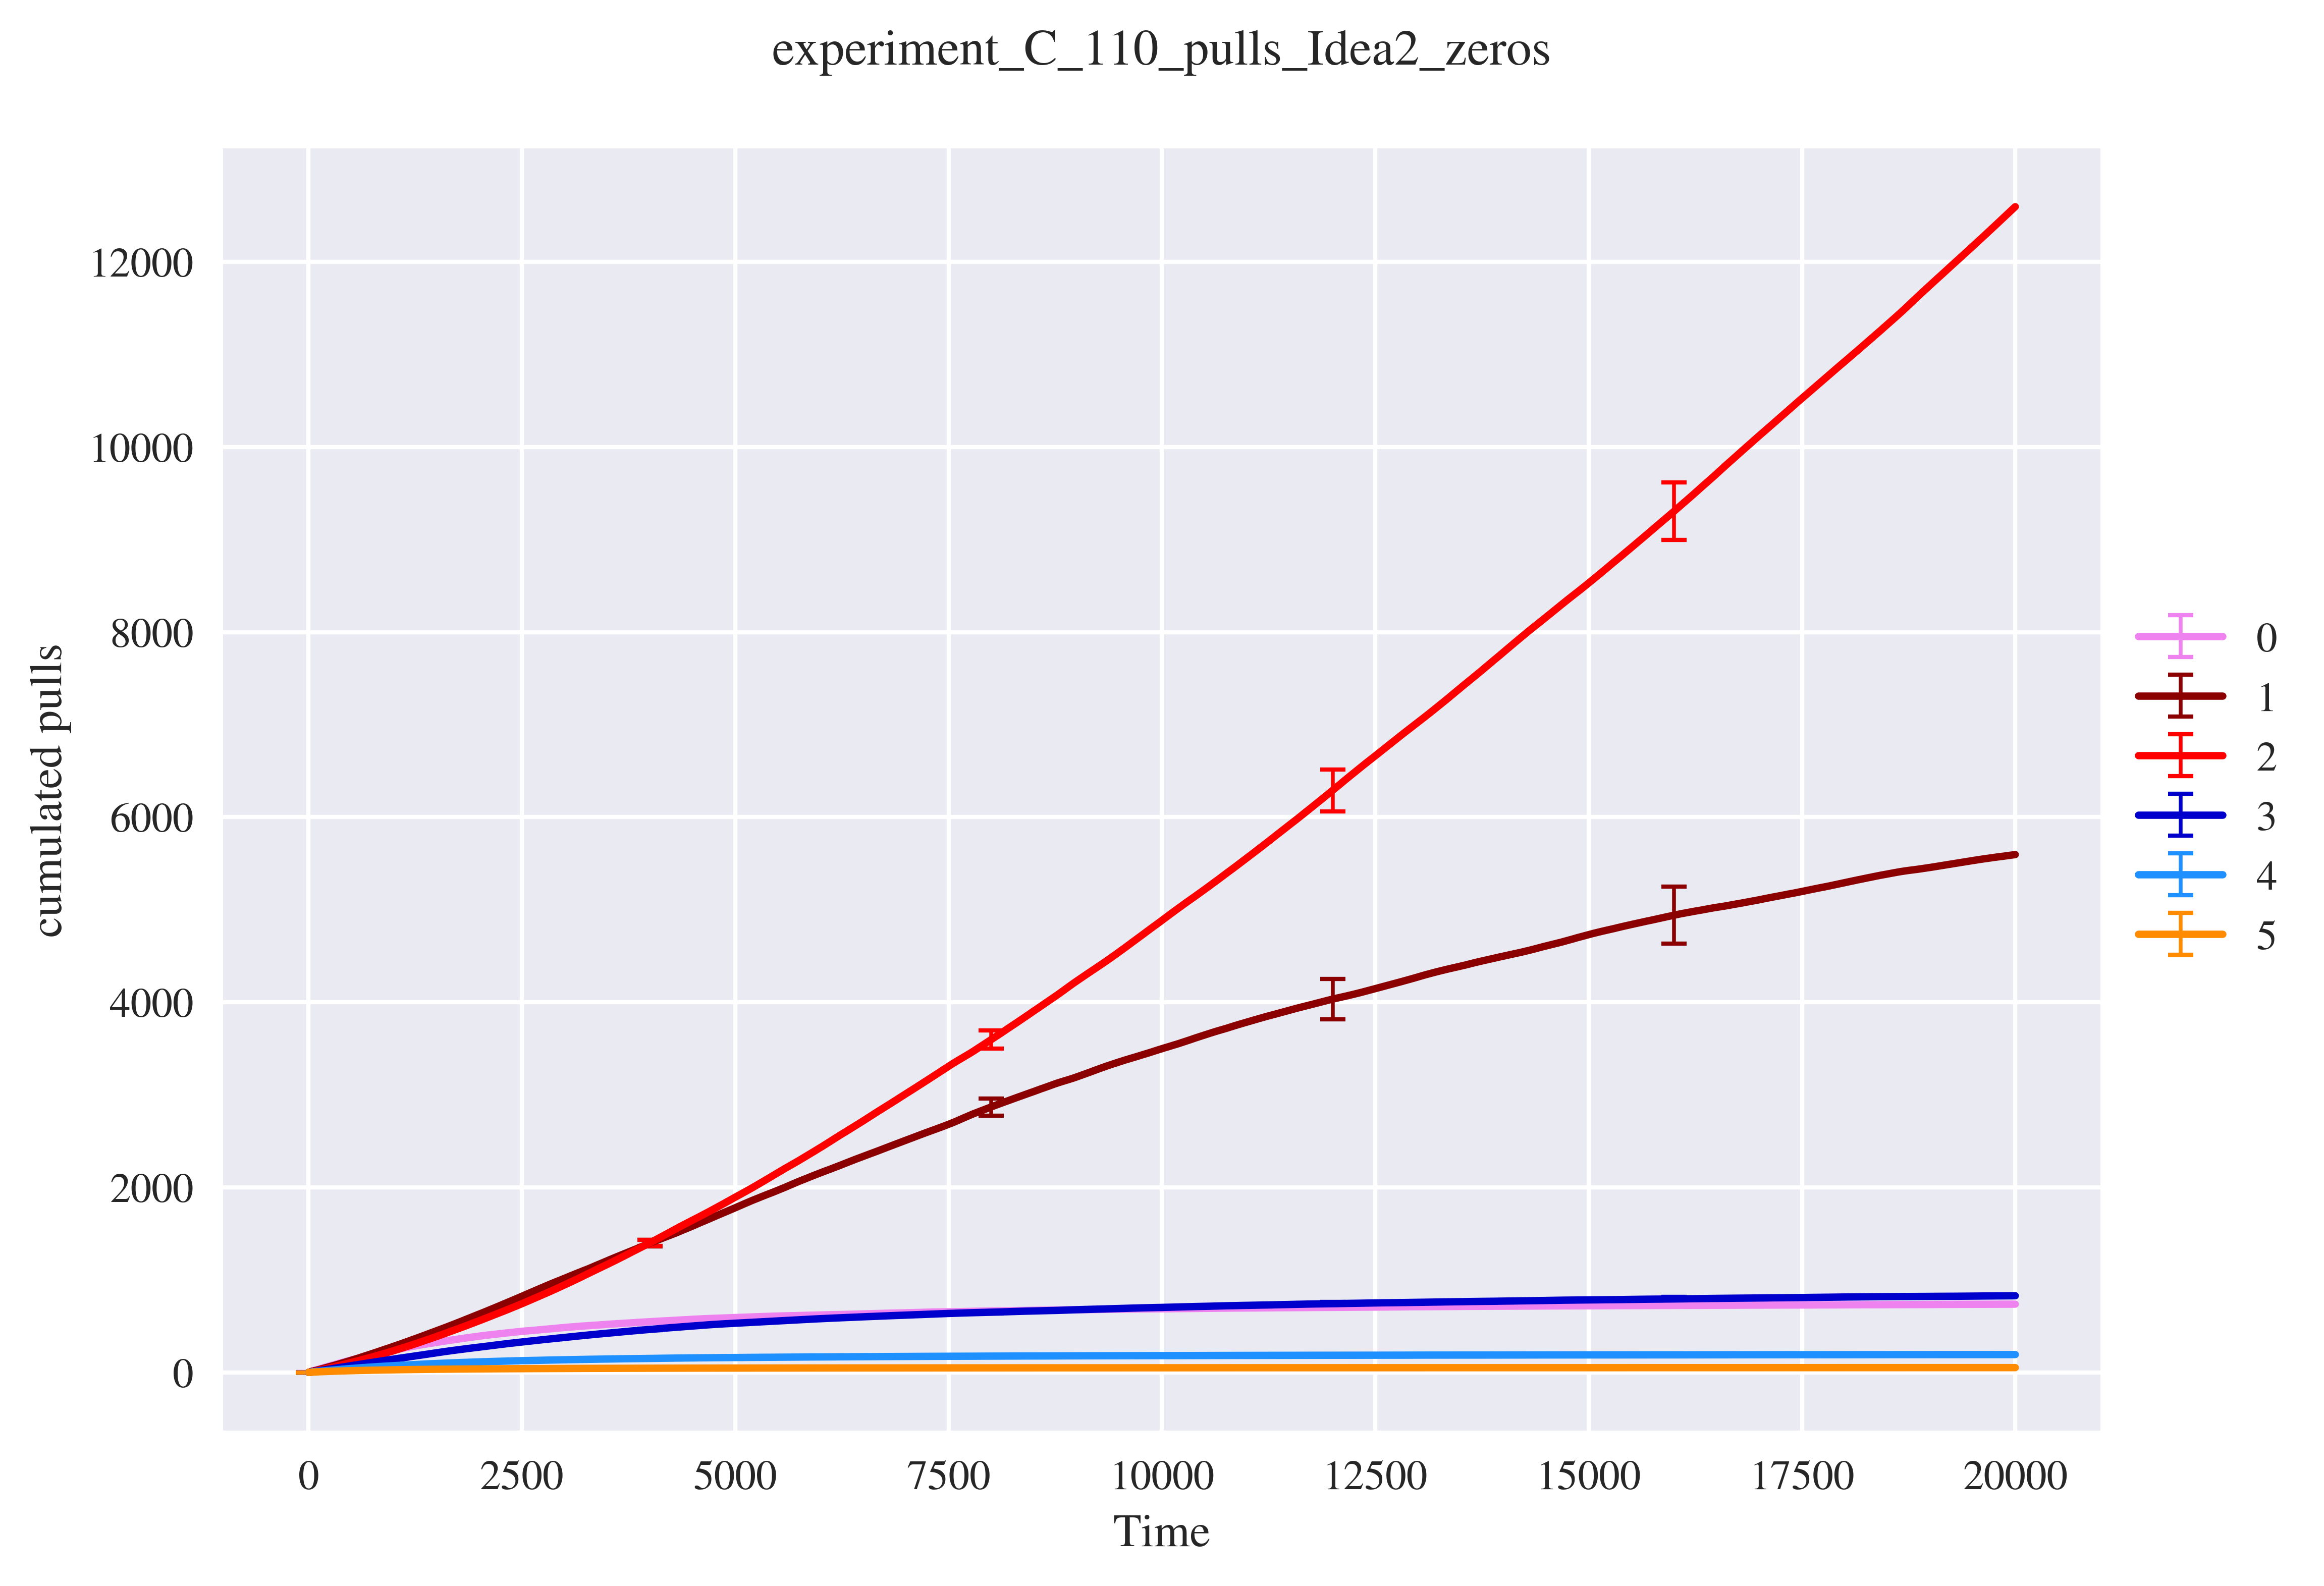
\includegraphics[width=6cm]{./images/PULLS/experiment_C_110Idea2_zeros cum_pulls.png}
	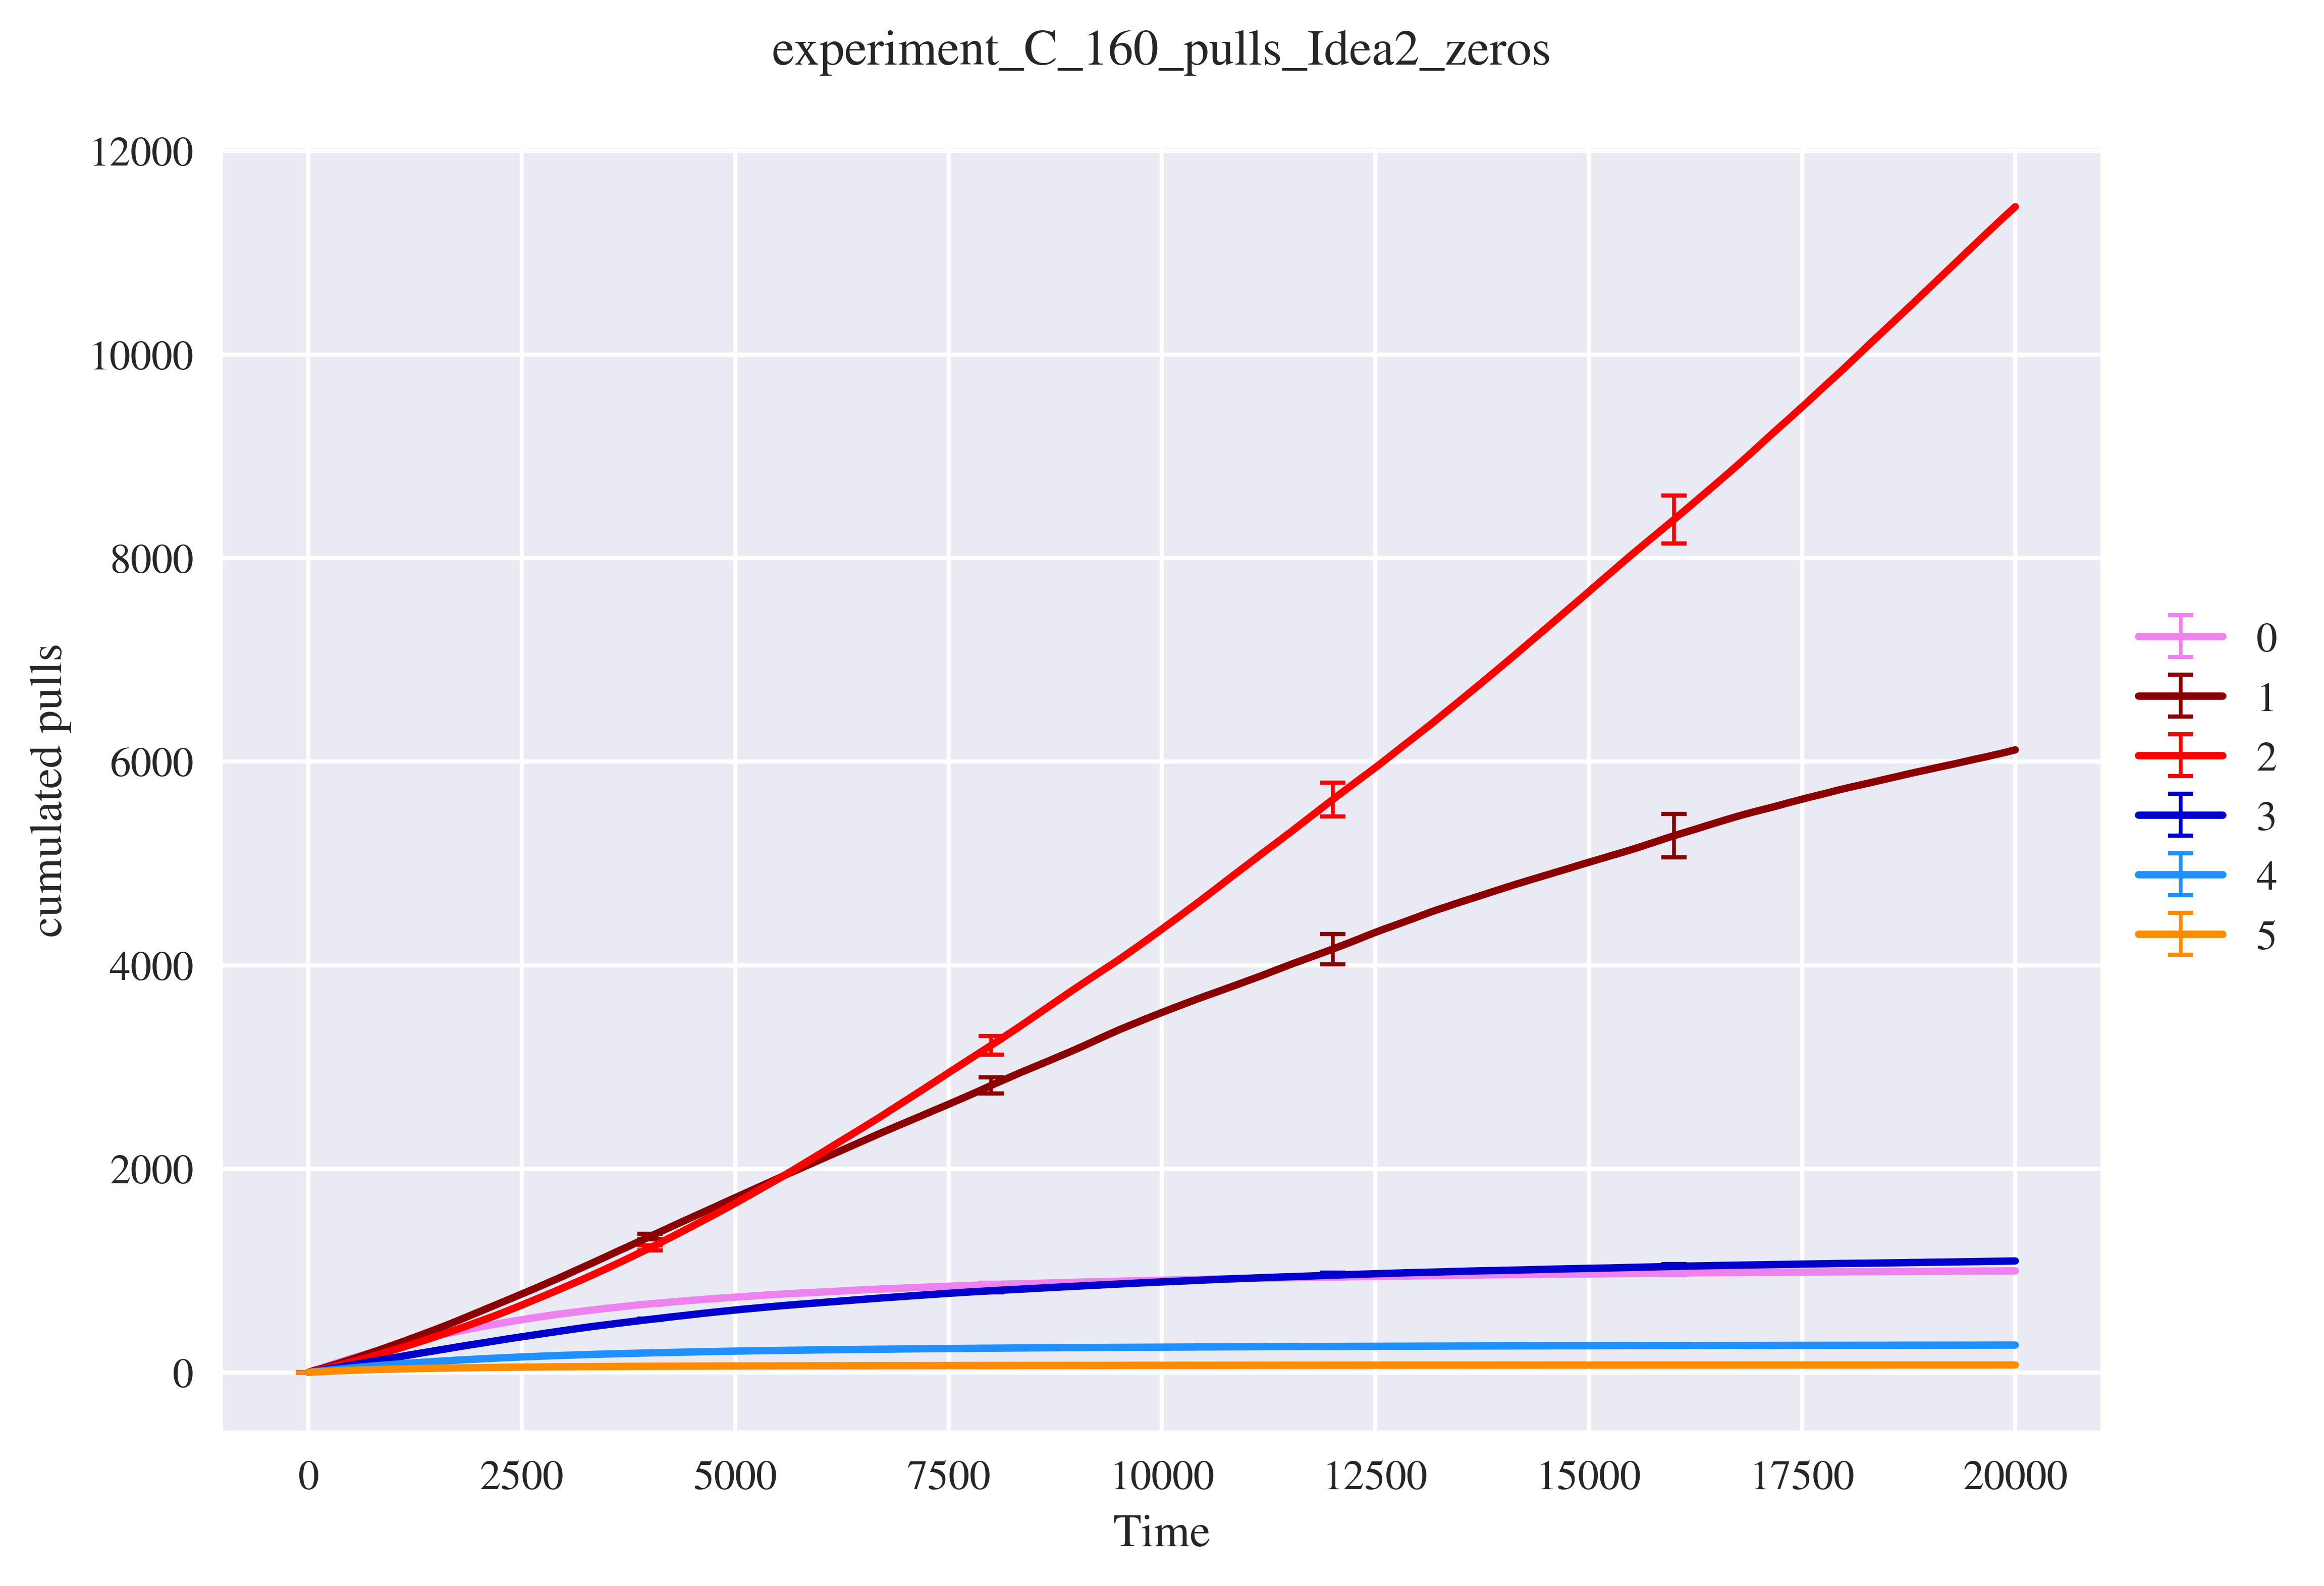
\includegraphics[width=6cm]{./images/PULLS/experiment_C_160Idea2_zeros cum_pulls.png}\quad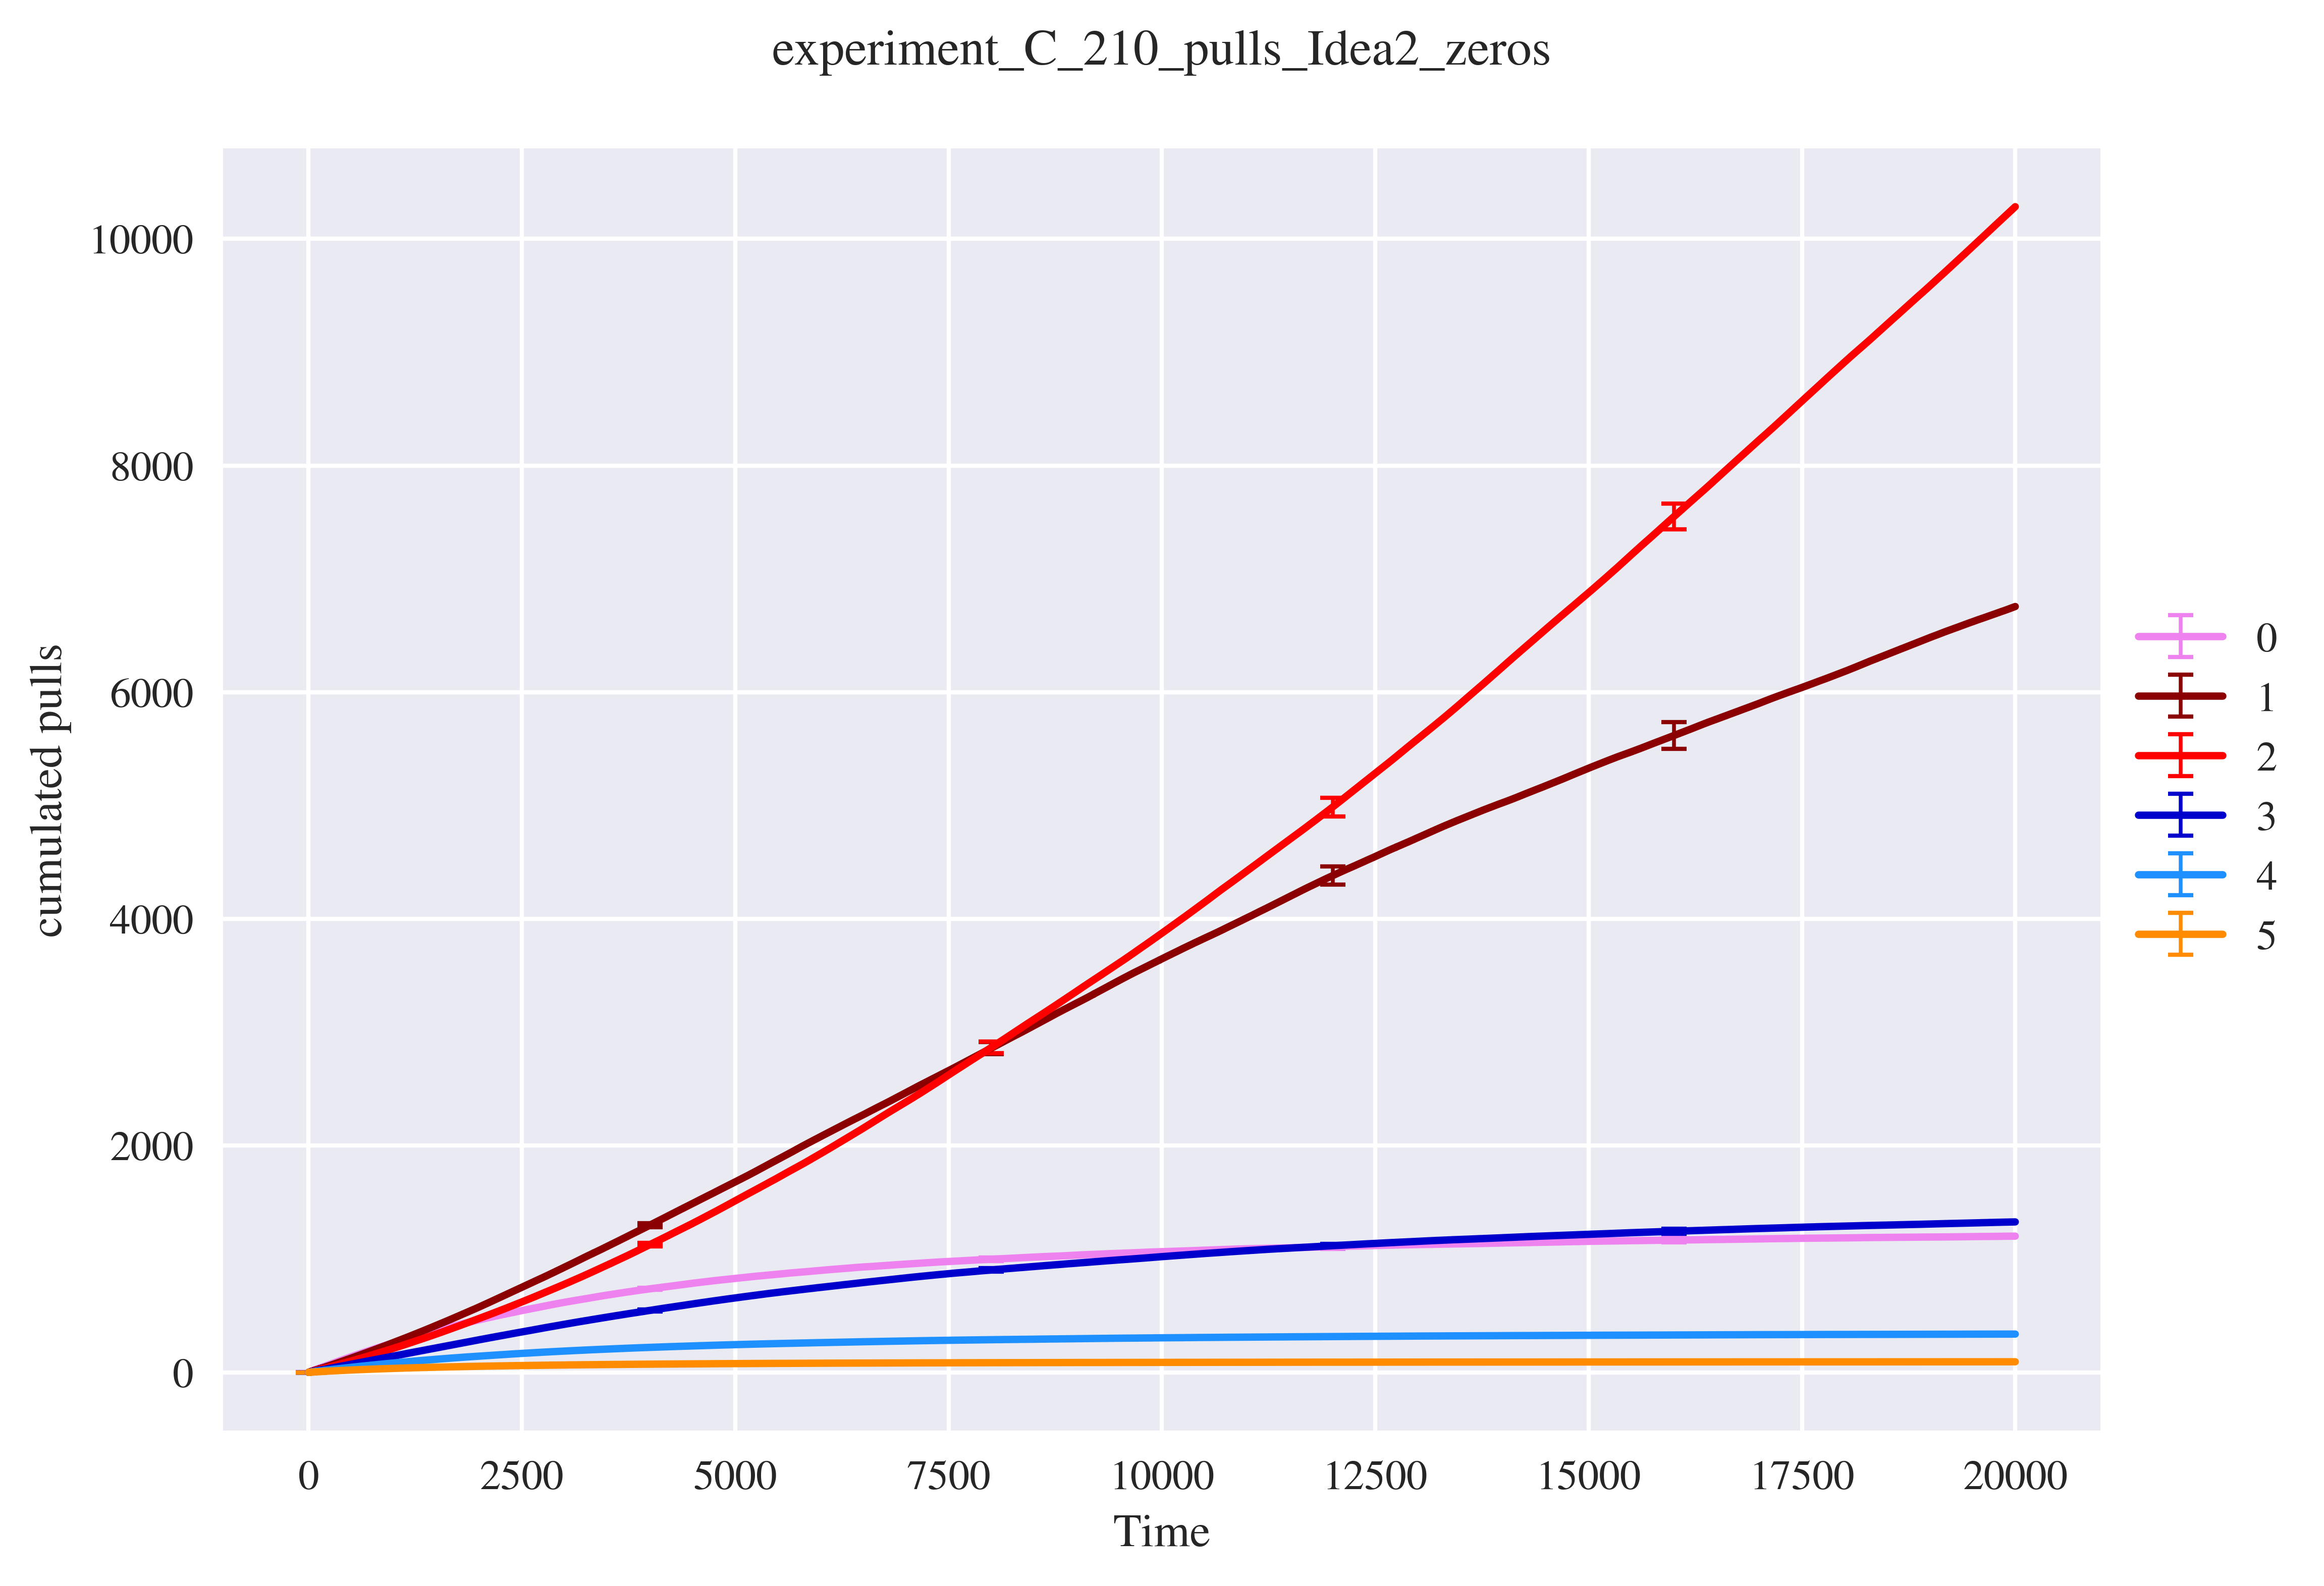
\includegraphics[width=6cm]{./images/PULLS/experiment_C_210Idea2_zeros cum_pulls.png}

	\caption{PULLS IDEA2 ZEROS C}
	
\end{figure}
